%% CEUR-WS / DL 2026 format
\documentclass[
% twocolumn,
% hf,
]{ceurart}

\sloppy

%% (DL logo removed for standalone version)

%%% Additional packages
\usepackage{amsmath,amssymb,amsthm}
\usepackage{booktabs}
\usepackage{enumitem}
\usepackage{xcolor}
\usepackage{graphicx}
\usepackage{tikz}
\usetikzlibrary{positioning}

%%% Theorem environments
\newtheorem{theorem}{Theorem}[section]
\newtheorem{lemma}[theorem]{Lemma}
\newtheorem{proposition}[theorem]{Proposition}
\newtheorem{corollary}[theorem]{Corollary}
\theoremstyle{definition}
\newtheorem{definition}[theorem]{Definition}
\newtheorem{examplex}[theorem]{Example}
\newtheorem{remark}[theorem]{Remark}

%%% Notation macros
\newcommand{\ALCI}{\ensuremath{\mathcal{ALCI}}}
\newcommand{\ALC}{\ensuremath{\mathcal{ALC}}}
\newcommand{\ALCIRCC}[1]{\ensuremath{\mathcal{ALCI}_{\mathit{RCC#1}}}}
\newcommand{\LRCC}[1]{\ensuremath{L_{\mathit{RCC#1}}}}
\newcommand{\DR}{\ensuremath{\mathsf{DR}}}
\newcommand{\PO}{\ensuremath{\mathsf{PO}}}
\newcommand{\EQ}{\ensuremath{\mathsf{EQ}}}
\newcommand{\PP}{\ensuremath{\mathsf{PP}}}
\newcommand{\PPI}{\ensuremath{\mathsf{PPI}}}
\newcommand{\TPP}{\ensuremath{\mathsf{TPP}}}
\newcommand{\NTPP}{\ensuremath{\mathsf{NTPP}}}
\newcommand{\TPPI}{\ensuremath{\mathsf{TPPI}}}
\newcommand{\NTPPI}{\ensuremath{\mathsf{NTPPI}}}
\newcommand{\DC}{\ensuremath{\mathsf{DC}}}
\newcommand{\EC}{\ensuremath{\mathsf{EC}}}
\newcommand{\inv}{\ensuremath{\mathsf{inv}}}
\newcommand{\comp}{\ensuremath{\mathsf{comp}}}
\newcommand{\cl}{\ensuremath{\mathsf{cl}}}
\newcommand{\Tp}{\ensuremath{\mathsf{Tp}}}
\newcommand{\Safe}{\ensuremath{\mathsf{Safe}}}
\newcommand{\md}{\ensuremath{\mathsf{md}}}
\newcommand{\Core}{\ensuremath{\mathsf{Core}}}
\newcommand{\Out}{\ensuremath{\mathsf{Out}}}
\newcommand{\Front}{\ensuremath{\mathsf{Front}}}
\newcommand{\EXPTIME}{\textsc{ExpTime}}
\newcommand{\PSPACE}{\textsc{PSpace}}
\newcommand{\naturals}{\mathbb{N}}
\newcommand{\reals}{\mathbb{R}}
\newcommand{\RCCfive}{\{\DR,\PO,\PP,\PPI\}}
%% Round-7 pair-shape / incidence-tag notation
\newcommand{\Q}{\ensuremath{\mathcal Q}}
\newcommand{\U}{\ensuremath{\mathcal U}}
\newcommand{\Pos}{\ensuremath{\mathsf{Pos}}}
\newcommand{\Pair}{\ensuremath{\mathsf{Pair}}}
\newcommand{\Tri}{\ensuremath{\mathsf{Tri}}}
\newcommand{\Base}{\ensuremath{\mathsf{B}}}
\newcommand{\lab}{\operatorname{lab}}
\newcommand{\self}{\ensuremath{\mathsf{self}}}
\newcommand{\eqtag}{\ensuremath{\mathsf{eq}}}
\newcommand{\up}{\ensuremath{\mathsf{up}}}
\newcommand{\down}{\ensuremath{\mathsf{down}}}
\newcommand{\side}{\ensuremath{\mathsf{side}}}
\newcommand{\front}{\ensuremath{\mathsf{front}}}

\begin{document}

%%
%% Rights management information.
\copyrightyear{2026}
\copyrightclause{Copyright for this paper by its authors.
  Use permitted under Creative Commons License Attribution 4.0
  International (CC BY 4.0).}

%%
%% Conference information (removed for standalone version)
%% \conference{DL 2026: 39th International Workshop on Description
%%   Logics, July 17--19, 2026, Lisbon, Portugal}

%%
%% Title
\title{On the Decidability of $\ALCIRCC{5}$:
  A Survey of the Problem, Its History, and a Proposed Solution}

%%
%% Authors
\author[1]{Michael Wessel}[%
email=miacwess@gmail.com,
url=https://github.com/lambdamikel,
]
\cormark[1]
\address[1]{University of Hamburg (doctoral work, 2002/2003)}

\author[2]{Claude (Anthropic)}[%
url=https://github.com/lambdamikel/alcircc5,
]
\address[2]{Anthropic, San Francisco, CA, USA}

\author[3]{GPT-5.4 (OpenAI)}[%
url=https://github.com/lambdamikel/alcircc5,
]
\address[3]{OpenAI, San Francisco, CA, USA}

\author[4]{GPT-5.5 (OpenAI)}[%
url=https://github.com/lambdamikel/alcircc5,
]
\address[4]{OpenAI, San Francisco, CA, USA}

\cortext[1]{Corresponding author.}

%%
%% Abstract
\begin{abstract}
The description logic $\ALCIRCC{5}$ extends $\ALCI$ with the five
RCC5 base relations as roles, under composition-table semantics.
Its decidability has been open since Wessel~(2002/2003).
We survey the history of the problem---from Cohn's original proposal
(1993) through Wessel's systematic investigation and Lutz \& Wolter's
related undecidability results (2006)---and explain why all known
undecidability reductions fail for $\ALCIRCC{5}$.
We then present a proposed decision procedure: the \emph{cover-tree
tableau}, which decomposes models into PPI-oriented cover trees
where only $\{\DR,\PO\}$ remain as open cross-edges.
This decomposition, combined with the patchwork property of RCC5,
yields finite blocking via rank-$d$ signatures.
The approach is supported by extensive computational evidence
(911~test concepts, zero mismatches; 775/775~SAT concepts with
cover-tree models) but has not been formally verified by human experts.
We discuss why na\"{\i}ve tableau approaches fail for
$\ALCIRCC{5}$ and how the cover-tree tableau overcomes these obstacles.
\end{abstract}

\begin{keywords}
  description logic \sep
  spatial reasoning \sep
  RCC5 \sep
  decidability \sep
  tableau calculus \sep
  patchwork property
\end{keywords}

\maketitle

%% ====================================================================
\section{Introduction}
\label{sec:intro}
%% ====================================================================

The decidability of concept satisfiability in the spatially extended
description logic $\ALCIRCC{5}$ has been an open problem for over
twenty years.  This paper provides a self-contained overview of the
problem, its intellectual history, the obstacles that have resisted
solution, and a proposed decision procedure that---if correct---would
settle the question positively.

The paper is organized as follows.
Section~\ref{sec:history} traces the history of $\ALCIRCC{5}$
from Cohn's original 1993 proposal through Wessel's systematic
investigation and Lutz \& Wolter's topological undecidability results.
Section~\ref{sec:undecidability} explains why standard undecidability
reductions fail, including a concrete domino-encoding attempt that
we verify is blocked.
Section~\ref{sec:naive-blocking} discusses why na\"{\i}ve tableau
approaches fail for complete-graph logics.
Section~\ref{sec:split-forest} presents the split-forest model
decomposition.
Section~\ref{sec:cover-tree} describes the cover-tree tableau and
explains how it achieves blocking.
Section~\ref{sec:outlook} concludes with an assessment of what
has been achieved and what remains to be done.

\textbf{Disclaimer.}
This paper was authored by AI assistants
(Claude Opus~4.7/Anthropic~\cite{ClaudeOpus47},
GPT-5.4~Pro/OpenAI~\cite{GPT54Pro}, and
GPT-5.5/OpenAI~\cite{GPT55Repaired}), prompted by Michael Wessel.
The results and proofs have \textbf{not been peer-reviewed or verified by
human domain experts}.  They are published as a discussion piece.
The claims should not be taken as established results unless independently
verified.  We invite scrutiny, corrections, and feedback.

%% ====================================================================
\section{History of $\ALCIRCC{5}$}
\label{sec:history}
%% ====================================================================

\subsection{Cohn's 1993 proposal}

The idea of combining description logics with qualitative spatial
reasoning via modal accessibility relations was first proposed by
Cohn~\cite{Cohn1993}, who considered treating the RCC8 relations
(or subsets thereof) as modalities in a multi-modal logic.
The framework allowed spatial constraints to be expressed as
modal formulas---e.g., $\langle \PP \rangle C$ for ``some proper
part satisfies~$C$''---but Cohn left all decidability and complexity
questions open.

\subsection{Wessel's $\ALCIRCC{}$ family (2002/2003)}

Wessel~\cite{Wessel2002,Wessel2003,Wessel2001} gave the first rigorous treatment
of the combination, introducing the \emph{$\ALCIRCC{}$ family}:
description logics $\ALCIRCC{k}$ ($k = 1,2,3,5,8$) extending $\ALCI$
with role boxes derived from the RCC composition tables.
In an $\ALCIRCC{k}$ interpretation, every pair of domain elements is
assigned exactly one RCC$k$ base relation, and the composition table
is enforced globally (\emph{strong $\EQ$ semantics}: $\EQ$ is identity).
Models are complete graphs with RCC$k$ edge-colorings.

Wessel established the following:
\begin{itemize}
  \item \textbf{Decidable cases:} $\ALCIRCC{1}$, $\ALCIRCC{2}$,
    and $\ALCIRCC{3}$ are decidable, because their composition
    tables are deterministic or near-deterministic, admitting
    reduction to standard DL techniques.
  \item \textbf{Lower bounds:} $\ALCIRCC{5}$ is $\PSPACE$-hard;
    $\ALCIRCC{8}$ is $\EXPTIME$-hard.
  \item \textbf{Open:} The decidability of $\ALCIRCC{5}$ and
    $\ALCIRCC{8}$ was left as the central open problem.
\end{itemize}

In a series of companion reports, Wessel also mapped out the
decidability landscape for description logics with general
composition-based role inclusion axioms:
\begin{itemize}
  \item $\ALC_{\mathcal{RA}}$ (arbitrary role axioms) is
    \textbf{undecidable}, via reduction from the Post
    Correspondence Problem~\cite{Wessel2001RA}.
  \item $\ALC_{\mathcal{RA}}^\ominus$ (non-disjoint-roles
    variant) is also \textbf{undecidable}, via reduction from
    non-empty CFG intersection~\cite{Wessel2000RA}.
  \item $\ALC_{\mathcal{RA}_{SG}}$ (admissible role boxes:
    deterministic, functional, complete, and associative) is
    \textbf{decidable} (\EXPTIME-complete, via reduction to
    $\ALC$ with general TBoxes)~\cite{Wessel2000SG}; adding
    unqualified number restrictions ($\mathcal{ALCN}_{\mathcal{RA}_{SG}}$)
    makes it undecidable again.
\end{itemize}
$\ALCIRCC{5}$ sits precisely in the gap: its role box is
non-deterministic (unlike $\ALC_{\mathcal{RA}_{SG}}$) but
has the patchwork property (unlike
$\ALC_{\mathcal{RA}}/\ALC_{\mathcal{RA}}^\ominus$).

\begin{remark}[Key difficulties]
$\ALCIRCC{5}$ has none of the properties that standard DL
decidability proofs rely on:
(i)~no tree model property (models are complete graphs),
(ii)~no finite model property (some satisfiable concepts require
infinite models),
(iii)~a non-deterministic role box (multi-valued composition entries).
\end{remark}

For reference, the full RCC5 composition table is given in
Table~\ref{tab:comp}.  Reading: row = $S(b,c)$, column = $R(a,b)$,
entry = possible relations for $(a,c)$.

\begin{table}[ht]
\centering
\caption{The RCC5 composition table ($*$ = all five relations).}
\label{tab:comp}
\renewcommand{\arraystretch}{1.15}
\begin{tabular}{l|ccccc}
\toprule
$\comp$ & $\DR(a,b)$ & $\PO(a,b)$ & $\EQ(a,b)$ & $\PPI(a,b)$ & $\PP(a,b)$ \\
\midrule
$\DR(b,c)$ & $*$ & $\DR,\PO,\PPI$ & $\DR$ & $\DR,\PO,\PPI$ & $\DR$ \\
$\PO(b,c)$ & $\DR,\PO,\PP$ & $*$ & $\PO$ & $\PO,\PPI$ & $\DR,\PO,\PP$ \\
$\EQ(b,c)$ & $\DR$ & $\PO$ & $\EQ$ & $\PPI$ & $\PP$ \\
$\PP(b,c)$ & $\DR,\PO,\PP$ & $\PO,\PP$ & $\PP$ & $\PO,\EQ,\PP,\PPI$ & $\PP$ \\
$\PPI(b,c)$ & $\DR$ & $\DR,\PO,\PPI$ & $\PPI$ & $\PPI$ & $*$ \\
\bottomrule
\end{tabular}
\end{table}

\noindent
Key composition facts exploited in the cover-tree theory
(Sections~\ref{sec:split-forest}--\ref{sec:cover-tree}):
$\comp(\PP,\DR) = \{\DR\}$ and $\comp(\DR,\PPI) = \{\DR\}$
(DR rigidity);
$\comp(\PP,\PP) = \{\PP\}$ and $\comp(\PPI,\PPI) = \{\PPI\}$
(transitivity);
and $\comp(\DR,\PO) = \{\DR,\PO,\PP\}$
(PP can be \emph{forced} by composition and universal filtering;
see Example~\ref{ex:pp-forcing}).

\subsection{Wessel's grid constructions and the coincidence obstruction}
\label{sec:wessel-grid}

In his investigation of $\ALCIRCC{8}$~\cite{Wessel2003}, Wessel
made two important discoveries:

\medskip\noindent\textbf{1.\ Even-odd chains (Section~4.4.2).}
The $\TPP/\NTPP$ distinction in RCC8 allows the construction of
\emph{functional successor chains}: each node alternates between
$\mathit{even}$ and $\mathit{odd}$, and a node can distinguish its
direct $\TPPI$-successor from all indirect ones by parity.
Wessel used this to encode a binary $n$-bit counter, proving
$\ALCIRCC{8}$ is $\EXPTIME$-hard.

\medskip\noindent\textbf{2.\ The grid coincidence obstruction (Section~4.4.3,
Figure~11).}
Wessel constructed explicit RCC8 networks isomorphic to
$n \times n$ grids, using $\TPP$ for horizontal and vertical
successors.  However, he identified a fundamental obstacle to
encoding domino tilings: the \emph{coincidence condition}
$R_X \circ R_Y = R_Y \circ R_X$ (east-of-north equals
north-of-east) cannot be enforced by concept terms.
The composition table allows $\{PO, EQ, TPP, NTPP, TPPI, NTPPI\}$
at the coincidence point---too many options.  Wessel concluded:
\begin{quote}
``Even though these infinite models do exist, we have found no way
to \emph{enforce} the depicted model(s) by means of a concept term.''
\end{quote}
Wessel further observed that adding a hybrid logic binding operator
$\downarrow$ (nominals) would immediately yield undecidability,
confirming that the coincidence condition is the \emph{precise
boundary}.

These constructions---the even-odd chain, the grid encoding via
$\TPP/\NTPP$, and the identification of the coincidence gap as
the decisive obstacle---anticipated key technical ingredients of
the later Lutz--Wolter proof by three to four years.

\subsection{Lutz \& Wolter (2006)}

Lutz and Wolter~\cite{LutzWolter2006} studied \emph{modal logics
of topological relations}, denoted $\LRCC{8}$, $\LRCC{5}$, etc.
These have the same \emph{syntax} as $\ALCIRCC{}$ but are
interpreted over \emph{topological models}: the domain elements
are regular closed subsets of a topological space (typically~$\reals^n$).
They proved:
\begin{itemize}
  \item $\LRCC{8}$ is \textbf{undecidable} (domino tiling via
    functional $\TPP$-chains, with the grid coincidence forced
    by the geometry of $\reals^2$).
  \item $\LRCC{5}(\mathit{RS}^\exists)$ is \textbf{undecidable}
    (reduction from $S5^3$ via supremum regions).
  \item $\LRCC{5}(\mathit{RS})$ is \textbf{open}. Lutz and Wolter
    explicitly wrote (p.~31): ``Perhaps the most interesting
    candidate is $L_{RCC5}(RS)$ [\ldots] to which the reduction
    exhibited in Section~8 does not apply.''
\end{itemize}

The logic $\ALCIRCC{5}$ is exactly $\LRCC{5}(\mathit{RS})$:
arbitrary complete-graph models with composition-table semantics.
The problem has been recognized as open by leading researchers
since 2006.

%% ====================================================================
\section{Why Undecidability Reductions Fail}
\label{sec:undecidability}
%% ====================================================================

Undecidability proofs for description logics use a variety of
techniques: grid encoding ($\naturals \times \naturals$ domino
tiling, requiring functional roles or number restrictions),
reduction from the Post Correspondence Problem (PCP), reduction
from context-free grammar (CFG) intersection, or simulation of
$S5^3$ via geometric constructions.
$\ALCIRCC{5}$ lacks the features that each of these techniques
exploits: it has no functional roles, no number restrictions,
no arbitrary role box, and no geometric coincidence conditions.

\subsection{Blocked reduction routes}

\begin{table}[t]
\caption{Why standard undecidability reductions fail for $\ALCIRCC{5}$.}
\label{tab:blocked}
\begin{tabular}{p{3.0cm}p{3.8cm}p{3.5cm}}
\toprule
\textbf{Source Problem} & \textbf{Technique} & \textbf{Missing in $\ALCIRCC{5}$} \\
\midrule
$\naturals \times \naturals$ domino & Graded modalities + transitivity & Number restrictions \\
$\ALC_{\mathcal{RA}}$ \cite{Wessel2001RA} & Post Correspondence Problem & Arbitrary role axioms \\
$\ALC_{\mathcal{RA}}^\ominus$ \cite{Wessel2000RA} & Non-empty CFG intersection & Non-disjoint roles \\
$\ALCIRCC{8}$ (Wessel) & Grid via $\TPP/\NTPP$ & $\TPP/\NTPP$ distinction \\
$\LRCC{8}$ (Lutz--Wolter) & Domino via topological $\TPP$ & Grid coincidence \\
$\LRCC{5}(\mathit{RS}^\exists)$ & $S5^3$ via supremum regions & Supremum closure \\
\bottomrule
\end{tabular}
\end{table}

Table~\ref{tab:blocked} summarizes the blocked routes.
The \textbf{patchwork property} of RCC5 (Renz \& Nebel~\cite{RenzNebel1999})---local
(triple-wise) consistency implies global consistency for atomic
networks---actively resists grid encoding, since tiling reductions
require rigid global constraints that go beyond local consistency.

\subsection{A concrete domino attempt in $\ALCIRCC{5}$}
\label{sec:domino-attempt}

Can we encode a domino-like grid using $\PP/\PPI$ chains in RCC5?
Consider the concept:
\begin{align*}
  X \;=\; &\exists\PPI.\exists\PPI.C \;\sqcap\; \exists\PPI.\exists\PPI.D \\
  &\sqcap\; \forall\PPI.\forall\PPI.(\forall\PO.(\neg C \sqcap \neg D)
    \sqcap \forall\DR.(\neg C \sqcap \neg D) \\
  &\qquad\qquad\qquad\quad\;\;
    \sqcap\; \forall\PPI.(\neg C \sqcap \neg D)
    \sqcap \forall\PP.(\neg C \sqcap \neg D)) \\
  &\sqcap\; \forall\PPI.\exists\PPI.X
\end{align*}
The intent: each $X$-node has two $\PPI$-grandchildren colored $C$
and $D$ (the ``square''), and the universals isolate the colored
nodes from all non-$\EQ$ neighbors.  The recursive
$\forall\PPI.\exists\PPI.X$ forces infinite repetition.

\medskip\noindent\textbf{One level is satisfiable.}
Without the recursive conjunct, $X$ has a 3-element model:
$z \;\PP\; y \;\PP\; x$, with $z \in C \sqcap D$.
The two grandchildren are forced to be \emph{the same element}
($\EQ$ collapse): if $z_1 \neq z_2$, they would be related by
some $R \in \RCCfive$, and the universals would require $z_2 \notin D$
(firing $z_1$'s $\forall R.\neg C \sqcap \neg D$).
So $z_1 = z_2 \in C \sqcap D$, and the universals are vacuously
satisfied (the only neighbors of~$z$ are PP-predecessors, not
PO/DR/PPI-neighbors).

\medskip\noindent\textbf{Two levels is unsatisfiable.}
Adding $\forall\PPI.X$: the $\PPI$-child $y$ must itself satisfy~$X$
(without recursion), producing a new $C \sqcap D$-labeled element~$w$
as a $\PPI$-child of~$z$.  But $z$ is a $\PPI$-grandchild of~$x$,
and $x$'s universals fire: $z$'s $\PPI$-neighbor~$w$ must satisfy
$\neg C \sqcap \neg D$.  Yet $w \in C \sqcap D$.
\textbf{Contradiction.}

This was verified computationally: a simplified version
$X_1 = \exists\PPI.\exists\PPI.C \sqcap \forall\PPI^3.\neg C$
is SAT; $X_2 = X_1 \sqcap \forall\PPI.X_1$ is UNSAT.
The domino encoding collapses at depth~2 because the isolation
constraints from the grandparent level kill the colored elements
created by the recursive unfolding.

\begin{remark}
The failure is not accidental.  In $\ALCIRCC{5}$, the only way to
create ``functional'' successors is via $\PP/\PPI$ chains, but
$\comp(\PPI,\PPI) = \{\PPI\}$ makes these chains
\emph{transitive}---grandparent universals automatically propagate
to grandchildren, preventing the positional diversity needed for
grid encoding.  In $\ALCIRCC{8}$, the $\TPP/\NTPP$ distinction
breaks this transitivity (a direct $\TPPI$-child is distinguishable
from indirect descendants), which is why Wessel's even-odd chain
works there but has no RCC5 analogue.
\end{remark}

\subsection{A concrete domino attempt in $\ALCIRCC{8}$}
\label{sec:domino-attempt-rcc8}

The remark above suggests the $\TPPI/\NTPPI$ distinction in
$\ALCIRCC{8}$ might rescue the construction: a direct successor
($\TPPI$) and an indirect one ($\NTPPI$) are genuinely
distinguishable, so perhaps the level-2 collapse can be avoided.
We attempt the analogue and show that while it escapes the RCC5
failure mode, it fails for a different reason---Wessel's
\emph{coincidence obstruction}~\cite{Wessel2003}.

\medskip\noindent\textbf{The schema.} Let $\textsf{Corner}$ be the
concept that isolates a node from all non-$\EQ$ neighbors:
\[
  \textsf{Corner} \;=\;
  \bigwedge_{R \,\in\, \{\DC,\EC,\PO,\TPP,\NTPP,\TPPI,\NTPPI\}}
    \forall R.(\neg C \sqcap \neg D).
\]
The isolation is placed \emph{locally on the colored grandchildren}
rather than as an ancestral $\forall\TPPI.\forall\TPPI$ universal,
so it cannot propagate transitively through the recursion:
\begin{align*}
  X \;=\; &\exists\TPPI.\exists\TPPI.(C \sqcap \textsf{Corner})
    \;\sqcap\; \exists\TPPI.\exists\TPPI.(D \sqcap \textsf{Corner}) \\
  &\sqcap\; \forall\TPPI.(\neg C \sqcap \neg D)
    \;\sqcap\; \forall\TPPI.X.
\end{align*}
The third conjunct $\forall\TPPI.(\neg C \sqcap \neg D)$ forces the
corner relation $x \to z$ to be $\NTPPI$ (not $\TPPI$), using
$\comp(\TPPI,\TPPI) = \{\TPPI, \NTPPI\}$.

\medskip\noindent\textbf{Level 1 is satisfiable, with a real
direct/indirect distinction.} Without recursion, $x$ has
$\TPPI$-children $y_1, y_2$ (the two ``direct'' positions) and a
single corner $z$ reached by $\TPPI$-$\TPPI$ chains from both
$y_1$ and $y_2$.  The EQ-collapse at level~2 works exactly as
in RCC5: $z_1 \in C \sqcap \textsf{Corner}$ and $z_2 \in D \sqcap
\textsf{Corner}$ are mutual non-$\EQ$ neighbors only if
$\textsf{Corner}$ is violated, so under strong-$\EQ$ semantics
$z_1 = z_2 = z$.  Crucially, $z \neq y_1, y_2$ in general: $z$ is
$\NTPPI$ of $x$ while $y_1, y_2$ are $\TPPI$---the direct/indirect
distinction survives, which is a genuine RCC8 refinement over the
RCC5 attempt of~\S\ref{sec:domino-attempt}.

\medskip\noindent\textbf{Level 2 collapses via the coincidence
obstruction.} Adding $\forall\TPPI.X$: the $\TPPI$-child $y$ of
$x$ satisfies $X$, producing its own corner $w \in C \sqcap D
\sqcap \textsf{Corner}$ at $\NTPPI$-distance from $y$, and hence
at $\NTPPI$-distance from $x$ via
$\comp(\TPPI, \NTPPI) = \{\NTPPI\}$.  Now $x$'s own corner $z$ and
$y$'s corner $w$ are distinct grid positions in the intended
reading---but as elements of the model they are related by some
RCC8 base relation.  Since $z$ carries $\textsf{Corner}$, every
non-$\EQ$ neighbor of $z$ lies in $\neg C \sqcap \neg D$.  But
$w \in C \sqcap D$.  Therefore $z = w$ under strong-$\EQ$.
\textbf{All corners across the grid coincide at a single point.}

\medskip\noindent\textbf{Why the $\TPPI/\NTPPI$ trick fails.} In
the RCC5 attempt the collapse is a \emph{transitive-propagation}
failure: the grandparent universal fires on great-grandchildren
because $\comp(\PPI,\PPI) = \{\PPI\}$.  Moving the isolation to a
local $\textsf{Corner}$ marker and using the non-transitive piece
$\comp(\TPPI,\TPPI) = \{\TPPI, \NTPPI\}$ eliminates that specific
pathway---the universal at the grandparent no longer reaches
deeper nodes.  But a \emph{different} obstruction takes over: the
composition table permits any of
$\{\PO, \EQ, \TPP, \NTPP, \TPPI, \NTPPI\}$ between two corners at
different intended grid coordinates, and nothing in the concept
language rules out $\EQ$.  The $\textsf{Corner}$ markers themselves
then force the EQ-merge.  This is exactly the obstruction Wessel
identified in report7.pdf, Figure~11 (cf.~\S\ref{sec:wessel-grid}):
the composition table does not carry the rigidity needed to keep
distinct grid cells distinct.

\begin{remark}
The failure mode is structurally different from the RCC5 one but
traces back to the same root cause.  Lutz--Wolter's $\LRCC{8}$
reduction resolves the coincidence obstruction using topological
geometry of $\reals^2$: east-of-north coincides with north-of-east
as a geometric fact, and each grid cell is a 2D region whose
boundary inclusions force distinct corners to be genuinely
distinct~\cite{LutzWolter2006}.  No such rigidity is available in
the abstract RCC8 semantics of $\ALCIRCC{8}$: a pure composition
table allows corner points to merge freely, and the $\TPPI/\NTPPI$
distinction---while useful locally for a direct/indirect
separation at level~2---cannot be chained to enforce an unbounded
$\naturals \times \naturals$ grid.  This matches the open-problem
status of $\ALCIRCC{8}$ decidability noted in~\cite{LutzWolter2006}
and further discussed in~\cite{Wessel2003}.
\end{remark}

%% ====================================================================
\section{Why Na\"{\i}ve Tableau Blocking Fails}
\label{sec:naive-blocking}
%% ====================================================================

Standard DL tableau calculi achieve termination through
\emph{blocking}: if a node~$x$ has the same label as an ancestor~$y$,
we can reuse $y$'s subtree for~$x$, cutting off infinite
branches.  The key requirement is that the ``reuse'' preserves
all constraints---in tree-shaped models, a blocked node's
interactions are limited to its parent edge, so label equality suffices.

In $\ALCIRCC{5}$, models are \emph{complete graphs}: every pair
of domain elements is related by an RCC5 base relation.
A node interacts not just with its parent and children, but with
\emph{every other node in the model}.
This creates a fundamental obstacle for blocking.

\begin{examplex}[Blocking breaks with cross-edges]
\label{ex:blocking-fail}
Consider $C_0 = \exists\PPI.A \sqcap \exists\DR.\neg A
\sqcap \exists\PO.\top$.
A tableau might generate nodes:
\begin{itemize}[nosep]
  \item $x_0$: root, satisfies $C_0$
  \item $x_1$: $\PPI$-child of $x_0$, type contains $A$
  \item $x_2$: $\DR$-witness for $x_0$, type contains $\neg A$
\end{itemize}
Now $x_1$ and $x_2$ must be related by some RCC5 relation~$R$,
and $R$ must be safe for their types.  If $x_1$ generates a
descendant $x_3$ with the same label as $x_1$, na\"{\i}ve blocking
would declare $x_3$ blocked.  But $x_3$'s relation to~$x_2$ may
differ from $x_1$'s relation to~$x_2$: via composition,
$\comp(\inv(\PPI), \DR) = \comp(\PP, \DR) = \{\DR\}$ forces
$x_1$ to be $\DR$-related to~$x_2$, while $x_3$ (deeper in the
tree) may face a different forced relation.  The blocked node's
cross-edge commitments differ from the blocking node's.
\end{examplex}

Multiple sophisticated blocking strategies have been tried and
failed for $\ALCIRCC{5}$~\cite{ALCIRCC5Outdated,StatusAfterFW,ResponseGPTBlocking}:
\begin{enumerate}
  \item \textbf{Profile-cached blocking} (GPT-5.4)~\cite{ResponseGPTBlocking}: Caches
    ``coherent predecessor blocks'' to compare global neighborhoods.
    Fails because the \emph{color structure changes during
    unraveling}---when a blocked subtree is replayed, the
    edge-coloring to nodes outside the subtree is not preserved.
  \item \textbf{Meet-semilattice replay} (GPT-5.4)~\cite{ResponseGPTBlocking}: Uses a
    meet-semilattice structure on labels to ensure robust
    normalization.  Same unraveling gap.
  \item \textbf{Tri-neighborhood blocking} (Claude)~\cite{TriangleBlocking}: Matches not
    just node labels but entire \emph{triangle neighborhoods}
    (the set of all types of 2-element subsets involving the node).
    \textbf{Termination disproved}: frontier nodes continuously
    acquire new triangle types as new neighbors are added, so
    $\mathrm{Tri}(x) \subsetneq \mathrm{Tri}(y)$ for frontier~$x$
    and interior~$y$---blocking never triggers.
  \item \textbf{Finite-witness / patchwork-augmentation probes}
    (Claude)~\cite{FWProof,PatchworkAugmentation,TypedPatchworkCounterexample}:
    Probes of a finite-witness conjecture and typed-patchwork
    augmentations for the contextual tableau, both refuted by
    explicit counterexamples.
\end{enumerate}

The common obstacle is the \textbf{blocking dilemma}: making the
blocking condition strong enough for soundness (matching all
cross-edge interactions) prevents termination (the cross-edge
context keeps growing), and vice versa.  A full catalogue of
retracted approaches is maintained
in~\cite{ALCIRCC5Outdated}; the overall project is summarised at
the repository~\cite{ALCIRCC5Repo}.

%% ====================================================================
\section{Split-Forest Model Decomposition}
\label{sec:split-forest}
%% ====================================================================

The breakthrough insight, due to Wessel, is to decompose
$\ALCIRCC{5}$ models into a \emph{tree layer} and a
\emph{cross-edge layer}, where the cross-edge layer is simple
enough to handle without full global blocking.
Figure~\ref{fig:whiteboard} reproduces the original whiteboard
sketch from April~7, 2026:\@ $\PPI$ chains form trees, $\DR/\PO$
are sibling cross-edges, and $\DR$ propagates rigidly downward
along $\PP$-chains.

\begin{figure}[ht]
\centering
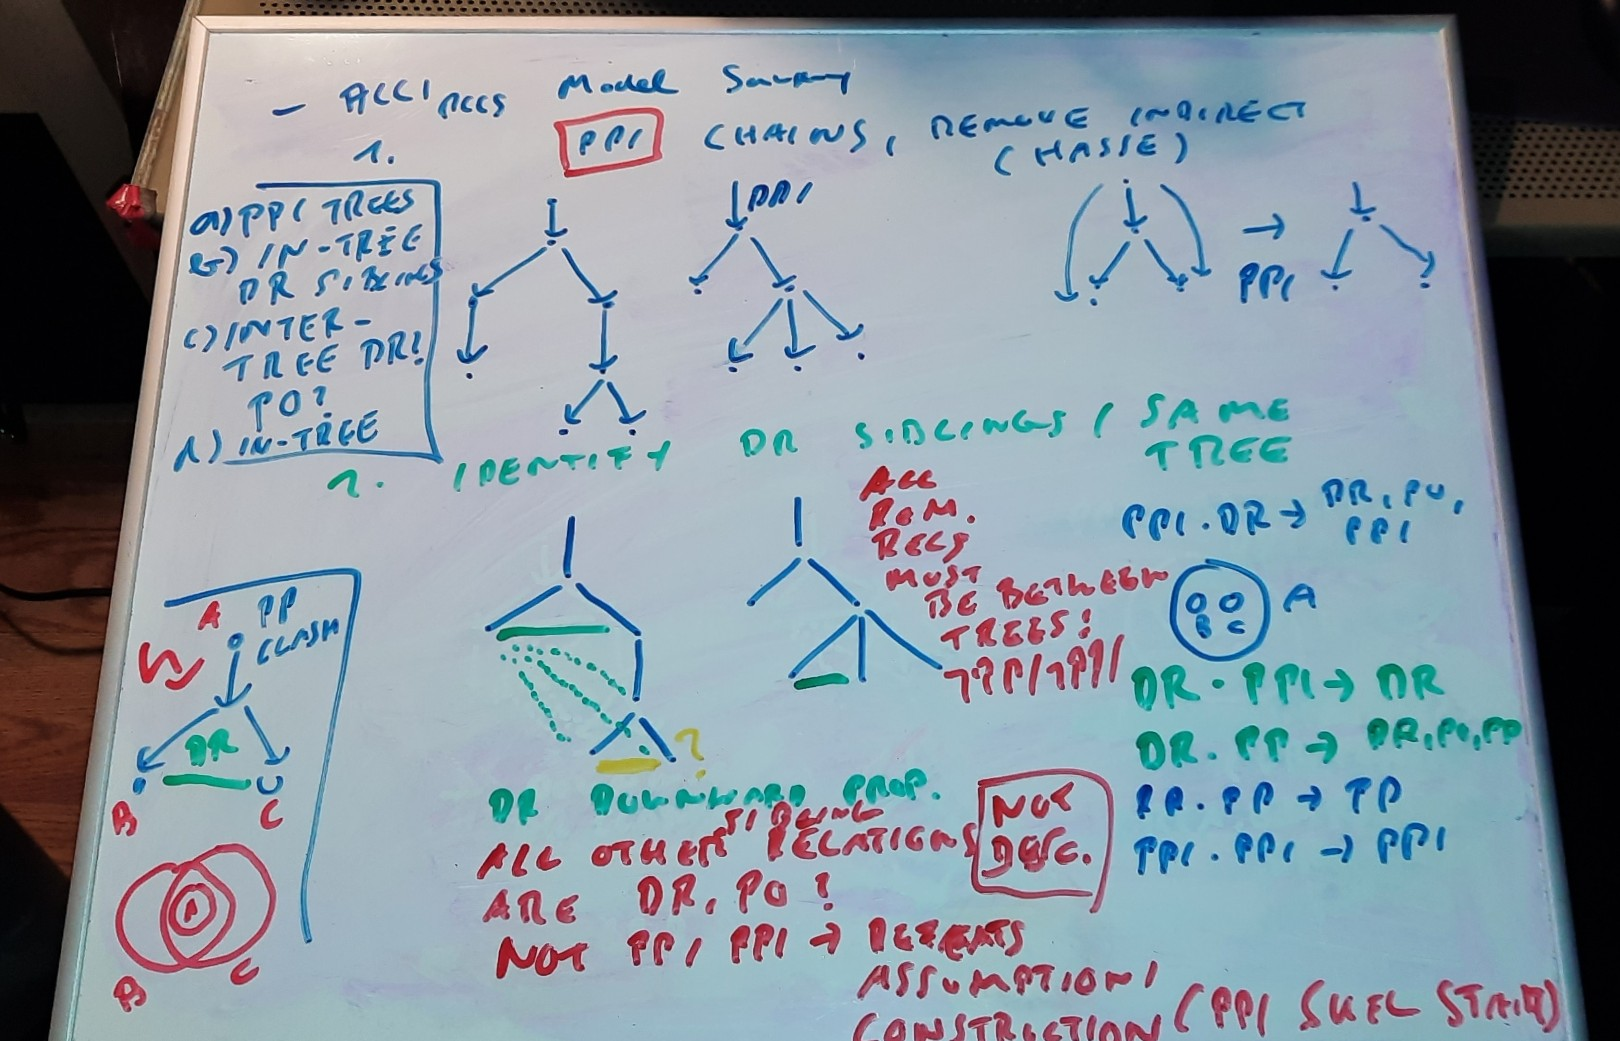
\includegraphics[width=0.85\columnwidth]{20260407_062616.jpg}
\caption{Wessel's whiteboard sketch (April~7, 2026) of the
  split-forest decomposition for $\ALCIRCC{5}$.  Vertical
  $\PPI$-chains form the cover-tree backbone (with join nodes
  split into $\EQ$-mates); $\DR/\PO$ become sibling cross-edges
  between non-comparable subtrees; and $\DR$ propagates rigidly
  downward because $\comp(\PP,\DR)=\comp(\DR,\PPI)=\{\DR\}$, so
  the residual cross-edge alphabet is just $\{\DR,\PO\}$, which
  is trivially arc-consistent.  Every subsequent formalisation
  in this paper---GPT-5.4's split-forest semantics, Claude's
  cover-tree tableau, and GPT-5.5's round-7 sketch---rests on
  this two-layer decomposition.}
\label{fig:whiteboard}
\end{figure}

\subsection{Cover trees}

In any $\ALCIRCC{5}$ model, the $\PP/\PPI$ relation is a
strict partial order (by composition: $\comp(\PP,\PP) = \{\PP\}$).
Orient this order downward ($\PPI$ = ``has proper part'') to
obtain a DAG.  If the DAG has join nodes (elements with multiple
$\PP$-predecessors), split them into $\EQ$-copies, one per parent
path.  The result is a rooted forest---the \emph{cover tree}.

\begin{definition}[Cover tree]
A \emph{cover-tree presentation} of an $\ALCIRCC{5}$ model
$\mathcal{I}$ is a rooted tree $T$ with a surjection
$\mathrm{orig}: T \to \Delta^{\mathcal{I}}$ such that:
(i) $u$ is the parent of $v$ in $T$ iff
$\mathrm{orig}(u) \;\PPI\; \mathrm{orig}(v)$ (immediate containment),
and (ii) tree nodes mapping to the same element are $\EQ$-mates
(weak-$\EQ$ semantics, convertible to strong-$\EQ$ by typed
congruence quotient).
\end{definition}

\subsection{The key observation: DR rigidity}

In the cover tree, what relations can hold between nodes in
different sibling subtrees?  Consider sibling roots $s$ and $t$
(children of the same parent), and elements $x$ below~$s$, $y$
below~$t$ in the tree.
An element~$x$ below~$s$ is in the \emph{$\Core$} of the sibling
pair $(s,t)$ if $\mathrm{orig}(x)$ is a common descendant of both
$\mathrm{orig}(s)$ and $\mathrm{orig}(t)$ in the original model's
$\PP$ order---i.e., $\mathrm{orig}(x)$ is a proper part of both.
Core elements are handled by $\EQ$-splitting; the interesting
question concerns non-$\Core$ elements.

\begin{proposition}[Wessel]
\label{prop:dr-rigid}
After $\EQ$-splitting, only $\DR$ and $\PO$ are possible between
non-$\Core$ elements of sibling subtrees.
\end{proposition}

\begin{proof}
\begin{itemize}[nosep]
  \item $\EQ(x,y)$: In the original DAG (before splitting),
    $x = y$ would mean a single element is a $\PP$-descendant of
    both $s$ and $t$---i.e., it is in the $\Core$.
    After splitting, this element is duplicated into
    distinct tree nodes $x'$ below~$s$ and $y'$ below~$t$,
    with $\mathrm{orig}(x') = \mathrm{orig}(y')$
    ($\EQ$-mates in the weak-$\EQ$ presentation).
    Since $x' \neq y'$ as tree nodes, $\EQ(x',y')$ is
    impossible under strong $\EQ$ semantics.
  \item $\PP(x,y)$: would mean $x$ lies below $y$ in the part-of
    order, hence below~$t$, making $x$ a common descendant
    ($\Core$).
  \item $\PPI(x,y)$: would place $y$ below~$x$ below~$s$, meaning
    $t$ lies below $s$---contradicting sibling incomparability.
\end{itemize}
Only $\DR$ and $\PO$ remain.  Furthermore, $\DR$ propagates
rigidly: $\comp(\PP, \DR) = \{\DR\}$ and $\comp(\DR, \PPI) = \{\DR\}$,
so if $s \;\DR\; t$, then \emph{every} descendant of~$s$ is $\DR$
to~$t$ and all its descendants.
\end{proof}

\subsection{Trivial arc-consistency of $\{\DR,\PO\}$ networks}

The consequence of Proposition~\ref{prop:dr-rigid} is that the
cross-edge constraint network uses only $\{\DR, \PO\}$ as possible
relations (plus $\{\DR\}$ for $\DR$-rigid pairs).

\begin{proposition}
\label{prop:drpo-arc}
For all $R, S \in \{\DR, \PO\}$:
$\comp(R, S) \cap \{\DR, \PO\} \neq \varnothing$.
\end{proposition}

This means a $\{\DR,\PO\}$ disjunctive network is
\emph{trivially arc-consistent}: every domain is either
$\{\DR\}$, $\{\PO\}$, or $\{\DR,\PO\}$, and composing any two
non-empty domains produces a non-empty result.
By the patchwork property~\cite{RenzNebel1999}, the network
therefore has a globally consistent atomic refinement whenever
every domain is non-empty.

This is the central simplification: \emph{checking that each type
pair has a non-empty $\{\DR,\PO\}$-safe set suffices for
cross-edge consistency.}  No full path-consistency computation is
needed.

%% ====================================================================
\section{The Cover-Tree Tableau}
\label{sec:cover-tree}
%% ====================================================================

\subsection{Algorithm overview}

The cover-tree tableau searches for a \emph{valid type set}:
a finite set $T \subseteq \Tp(C_0)$ of Hintikka types that
contains a root type realizing~$C_0$ and satisfies four conditions:

\begin{enumerate}[label=(CT\arabic*)]
  \item \textbf{Demand closure}: every existential demand
    $\exists R.D$ in every $\tau_i \in T$ has an $R$-safe
    witness $\tau_j \in T$ with $D \in \tau_j$.
  \item \textbf{Cross-edge consistency}: every pair
    $\tau_i, \tau_j \in T$ has either $\Safe(\tau_i,\tau_j)
    \cap \{\PP,\PPI\} \neq \varnothing$ (tree-relatable) or
    $\Safe(\tau_i,\tau_j) \cap \{\DR,\PO\} \neq \varnothing$
    (cross-relatable).
  \item \textbf{Cover-tree sibling compatibility}: for each
    type $\tau_i$ with multiple $\DR/\PO$ demands, the witnesses
    can be jointly assigned such that every witness pair satisfies
    $\comp(\inv(R_m), R_{m'}) \cap \{\DR,\PO\} \cap
    \Safe_{\DR/\PO}(\tau_{j_m}, \tau_{j_{m'}}) \neq \varnothing$.
  \item \textbf{Composition propagation}: for each type with
    multiple demands of \emph{any} role combination, witnesses
    $\tau_{j_1}, \tau_{j_2}$ must satisfy
    $\comp(\inv(R_1), R_2) \cap \Safe(\tau_{j_1}, \tau_{j_2})
    \neq \varnothing$.
\end{enumerate}

The algorithm terminates because $|\Tp(C_0)| \leq 2^{|\cl(C_0)|}$
is finite, and the type set grows monotonically during the search.

\subsection{How blocking works}

The crucial difference from na\"{\i}ve tableau approaches is the
\emph{separation of layers}:

\begin{itemize}
  \item The \textbf{tree layer} ($\PP/\PPI$) handles
    ancestor/descendant demands.  Since $\PP/\PPI$ form a tree,
    standard tree-model arguments apply: blocking via
    \emph{rank-$d$ signatures} (the type information visible
    within modal depth~$d = \md(C_0)$) yields a finite
    representation.

  \item The \textbf{cross layer} ($\DR/\PO$) handles demands for
    disconnected or partially overlapping regions.  Because the
    cross-edge network uses only $\{\DR,\PO\}$---which is
    trivially arc-consistent---the cross-layer check reduces to a
    simple pairwise non-emptiness condition (CT2), not a global
    consistency computation.
\end{itemize}

Na\"{\i}ve blocking fails because it tries to handle both layers
simultaneously: the tree structure provides natural blocking, but
the cross-edges to distant nodes keep changing, preventing a match.
The cover-tree tableau sidesteps this by \emph{not} blocking on
cross-edge context---instead, it verifies cross-edge consistency
as a separate, global check on the finite type set.

\begin{examplex}[A concept that defeats na\"{\i}ve blocking but
  works with cover trees]
\label{ex:cover-tree-win}
Consider $C_0 = \exists\PO.A \sqcap \exists\PP.\neg B \sqcap
\forall\DR.A$.
In a na\"{\i}ve tableau, the $\PP$-child needs further expansion;
blocking requires matching both the label \emph{and} the
triangle neighborhood (relations to the $\PO$-witness and all
other nodes).  Since the $\PO$-witness forces $\DR$-relations
to the $\PP$-child's subtree (via $\comp(\PO, \PP) = \{\DR,\PO,\PP\}$),
the cross-edge context keeps evolving.

In the cover-tree tableau: the $\PP$-witness is an ancestor in
the tree, the $\PO$-witness is a cross-edge in a sibling subtree.
The $\forall\DR.A$ fires only on $\DR$-related nodes---the
ancestor is $\PP$-related (not $\DR$), so no conflict.
The type set $T$ needs a type for the root (containing $C_0$),
one for the $\PO$-witness (containing $A$), and one for the
$\PP$-witness (containing $\neg B$).  Cross-edge consistency
(CT2) checks that every pair has a non-empty safe set in
$\{\DR,\PO\}$---a one-time pairwise check, not an evolving
context.
\end{examplex}

\begin{examplex}[Implicit PP via composition forcing]
\label{ex:pp-forcing}
The concept
\[
  X \;=\; \exists\DR.\exists\PO.C
    \;\sqcap\; \forall\DR.\neg C
    \;\sqcap\; \forall\PO.\neg C
    \;\sqcap\; \forall\PP.X
\]
contains no $\exists\PP$ demand, yet it requires an infinite
model with forced $\PP$ edges.

A node~$r$ satisfying~$X$ has a $\DR$-neighbor~$a$
(with $\exists\PO.C$) and $a$'s $\PO$-neighbor~$b$
(with~$C$).  By Table~\ref{tab:comp}, the relation
between $r$ and $b$ lies in
$\comp(\DR,\PO) = \{\DR,\PO,\PP\}$.
But $r$ has $\forall\DR.\neg C$ and $\forall\PO.\neg C$,
and $b \in C$---so $\DR$ and $\PO$ are blocked, leaving
\emph{only}~$\PP$.  The $\PP$ edge is \textbf{forced} by
composition plus universal filtering, with no explicit
$\exists\PP$ in the concept.

Since $r \;\PP\; b$, node $b$ is an \emph{ancestor} of~$r$
in the cover tree.  The recursive $\forall\PP.X$ forces $b$
to also satisfy~$X$, creating its own
$\DR \to \PO$ chain and forcing yet another $\PP$-ancestor
above it:
\[
  r \;\PP\; b \;\PP\; b' \;\PP\; b'' \;\PP\; \cdots
\]
The model is necessarily infinite.  The cover-tree tableau
handles this finitely: the type for $C$-elements can serve as
its own $\PP$-ancestor (different domain elements, same
abstract state), so a three-element type set
$\{\tau_0(C,X),\; \tau_1(\neg C, \exists\PO.C),\;
  \tau_2(\neg C, \text{root})\}$
represents the infinite model.

This pattern---$\PP$ edges arising purely from composition and
universal filtering---is a distinctive feature of $\ALCIRCC{5}$
and illustrates why the complete-graph semantics require careful
handling of implicit spatial constraints.
\end{examplex}

\begin{examplex}[The ``$\PO$-loop'': 2-element SAT via symmetric cycles]
\label{ex:po-loop}
Naive reasoning suggests
\[
  Y \;=\; C
    \;\sqcap\; \exists\PO.\exists\PO.C
    \;\sqcap\; \forall\PO.\neg C
    \;\sqcap\; \forall\DR.\neg C
    \;\sqcap\; \forall\PP.\neg C
    \;\sqcap\; \forall\PPI.\neg C
\]
should be unsatisfiable: any witness chain
$d \;\PO\; a \;\PO\; b$ with $b \in C$ needs
$\rho(d,b) \in \comp(\PO,\PO) = \{\DR,\PO,\PP,\PPI,\EQ\}$,
and the four universals $\forall R.\neg C$ seem to block every
non-$\EQ$ option (each forces $b \in \neg C$, yet $b \in C$).

But $Y$ is in fact \textbf{satisfiable}, via the two-element model
$\{d,a\}$ with $C^{\mathcal I} = \{d\}$ and $\rho(d,a) = \PO$.
Because $\PO$ is symmetric
($\PO(d,a) \Rightarrow \PO(a,d)$), the chain
$d \;\PO\; a \;\PO\; d$ loops back to the root itself: the
``third node'' of the $\exists\PO.\exists\PO$ formula \emph{is}
$d$, under strong $\EQ$ identity. Two syntactic positions in the
nested existential map to the same semantic element.

The universals $\forall R.\neg C$ constrain $d$'s \emph{outgoing}
$R$-neighbours (the sole $\PO$-neighbour $a \in \neg C$
satisfies them), but they do \textbf{not} prevent $d$ from
\emph{being} a $\PO$-neighbour of $a$: the witness for $a$'s
$\exists\PO.C$ is $d$ itself, and $a$ has no
$\forall\PO$-constraint forbidding $C$-neighbours.
This asymmetry between ``constraints on my neighbours'' and
``constraints on what I may be a neighbour of'' is peculiar
to symmetric roles ($\PO,\DR$). The cover-tree tableau correctly
reports $Y$ as satisfiable.
\end{examplex}

\begin{examplex}[``Clash-out to $\EQ$'': genuine UNSAT via strong $\EQ$]
\label{ex:clash-to-eq}
The complementary pattern
\[
  Z \;=\; C
    \;\sqcap\; \exists\PO.\exists\PO.\neg C
    \;\sqcap\; \forall\PO.C
    \;\sqcap\; \forall\DR.C
    \;\sqcap\; \forall\PP.C
    \;\sqcap\; \forall\PPI.C
\]
\emph{is} unsatisfiable, and the reason is instructive. The chain
$d \;\PO\; a \;\PO\; c$ forces $a \in C$ (via $\forall\PO.C$ at $d$)
and $c \in \neg C$ (via $\exists\PO.\neg C$ at $a$). The
relation $\rho(d,c)$ must lie in
$\comp(\PO,\PO) = \{\DR,\PO,\PP,\PPI,\EQ\}$. The four universals
$\forall R.C$ at $d$ (for $R \in \{\DR,\PO,\PP,\PPI\}$) each
require $c \in C$, contradicting $c \in \neg C$, hence
\emph{all four non-$\EQ$ options are blocked}. Only $\EQ$ remains.

Under \textbf{strong $\EQ$ semantics} ($\EQ$ = identity),
$\rho(d,c) = \EQ$ forces $d = c$, yielding $d \in C \land d \in \neg C$
and a clash. The $\PO$-loop escape of
Example~\ref{ex:po-loop} does not apply here: the endpoint $c$
requires $\neg C$ while $d$ has $C$, so $d \ne c$ is forced
semantically, and the universals then close every non-$\EQ$
composition entry.

This example illustrates why \emph{strong} $\EQ$ semantics is
essential for our undecidability- and decidability-proof
machinery. Under weak $\EQ$ (equivalence-class) semantics,
collapsing $d$ and $c$ would not immediately clash, and one would
need additional machinery (equality propagation,
congruence-closure) to derive the same conclusion. The strong
reading is also the one built into the composition tables used
in Renz \& Nebel's patchwork theorem.
\end{examplex}

\begin{remark}[Reasoners and tools: a cross-validation suite]
\label{rem:tools}
This paper references three Python tools used in the companion
implementations; before the incompleteness below we fix their
roles. The \textbf{cover-tree tableau}
(\texttt{cover\_tree\_tableau.py}, Section~\ref{sec:cover-tree})
is the main candidate decision procedure---the only tool whose
soundness and completeness are claimed for $\ALCIRCC{5}$
satisfiability, resting on the patchwork property of RCC5 and
the companion completeness-extraction argument. The
\textbf{quasimodel reasoner}~\cite{QuasimodelReasoner}
(\texttt{alcircc5\_reasoner.py}, with cycle-aware wrapper
\texttt{alcircc5\_reasoner\_cyclic.py}) is a constructive
bottom-up quasimodel search based on disjunctive
path-consistency; it is used \emph{only} as a cross-validation
oracle for the cover-tree tableau, not as a step of any
decidability argument. The \textbf{independent model verifier}
(\texttt{model\_verifier.py}) grounds SAT answers in concrete
finite RCC5 models, separately checking inverse symmetry,
composition consistency on all triples, type-safety,
existential witnessing, and recursive concept truth. The three
tools together form a cross-validation suite around the
cover-tree tableau: cover-tree produces the candidate verdict,
the quasimodel reasoner offers an independent opinion, and the
model verifier anchors SAT answers in explicit models.
\end{remark}

\begin{remark}[Implementation-level bugs found and fixed in April 2026]
\label{rem:impl-bugs}
Three implementation-level defects were identified in April~2026
and fixed in the cover-tree tableau and the baseline quasimodel
reasoner: (i) the baseline quasimodel reasoner was incomplete on
cyclic-via-symmetric-role SAT concepts such as the
$\PO$-loop of Example~\ref{ex:po-loop} (closed by an opt-in
cycle-close clause in \texttt{alcircc5\_reasoner\_cyclic.py});
(ii) the shared \texttt{compute\_safe} helper failed to propagate
$\forall\PP/\PPI.D$ universals as a whole into successor types
(fixed by the standard transitive-role trick); (iii) the
cover-tree's pairwise tree-cross check missed twelve UNSAT
patterns of the form $\exists R_1.\exists R_2.A\sqcap
\bigwedge_{R\in\comp(R_1,R_2)}\forall R.\neg A$ when intermediate
types carry a single demand (fixed by porting the quasimodel
reasoner's role-path compatibility fixpoint as Phase~5 / (CT5)).
The decidability argument is unaffected by any of these fixes:
all three were soundness gaps in implementations of the
candidate decision procedure, not the split-forest /
completeness-extraction argument that underpins the theorem.
The $911$-concept cross-validation continues to match $911/911$
before and after every fix; full technical detail (root cause,
algebraic justification, regression tests) is in the cover-tree
implementation paper~\cite{CoverTreeImpl}.
\end{remark}

\subsection{What makes this ``non-standard''}

The cover-tree tableau differs from a standard DL tableau
calculus in several fundamental ways:

\begin{enumerate}
  \item \textbf{No completion graph.}  Standard tableaux build a
    completion graph node by node, applying expansion rules until
    saturation or clash.  The cover-tree tableau searches over
    \emph{sets of types} (abstract states), not concrete graph
    structures.  It is closer to a type-elimination or
    automata-theoretic approach.

  \item \textbf{No explicit blocking rule.}  Standard tableaux
    have an explicit blocking condition that compares nodes during
    expansion.  The cover-tree tableau achieves finiteness
    \emph{structurally}: the search space is the powerset of
    $\Tp(C_0)$, which is already finite.

  \item \textbf{Global side-checker.}  The cross-edge constraints
    (CT2--CT4) are checked globally over the entire type set,
    not locally during node expansion.  This is what avoids the
    blocking dilemma: cross-edge consistency is a property of
    the type set as a whole, not of individual nodes.

  \item \textbf{Existential demands go to ALL existing types.}
    In a standard tableau, $\exists R.D$ generates one new
    $R$-neighbor.  In the cover-tree tableau, the witness can
    be \emph{any} type already in~$T$---including the root type
    itself.  This reflects the complete-graph semantics: every
    domain element is related to every other.
\end{enumerate}

\subsection{Soundness and completeness}
\label{ssec:soundness-completeness}

The decidability theorem is established by the GPT-5.5 \emph{round-8
saturated-side-context split-forest
proof}~\cite{GPT55Round8Sketch} (May~2026, 15-page sketch,
no-automata route), with detailed
companion~\cite{GPT55Round8Expanded} (30~pages) and an independent
parity-tree-automata witness~\cite{GPT55AutomataRoute} (21~pages).
Round-8 preserves the round-7 architectural move (incidence-tagged
pair shapes) and adds three repairs identified by a cold Claude
review of round-7:\@ a \emph{saturated side context}
$S_k(u)$ in which equality- and containment-closure are applied
before the residual $\DR/\PO$ restriction, a
\emph{cross side/tree exhaustion lemma} ruling out hidden
$\PP/\PPI$ pairs between vertical-boundary positions and side
positions, and \emph{constructed pair and triple catalogues}
$\Pair_\Q,\Tri_\Q$ replacing the round-7 finiteness-only
assertions.  The history of how the proof reached its current
form is collected in~\S\ref{sec:history-of-attempts} below; this
subsection states the current result.

\paragraph{Soundness} (valid certificate $\Rightarrow$ strong
abstract RCC5 model satisfying $C_0$).  A finite split-forest
certificate $\Q$ is unfolded to an occurrence structure $\U(\Q)$
in which repeated cycle profiles generate fresh concrete
occurrences.  The quotient $\U(\Q)/\eqc$ by the explicit
equality-port congruence is a strong abstract RCC5 frame:
strong-$\EQ$ holds because the quotient identifies exactly
$\eqc$-classes; inverse symmetry and RCC5 composition hold because
the round-7 label function and triple-composition clause~(V6) are
verified on the finite occurrence-sensitive certificate.  A truth
lemma over $\Cl(C_0)$ shows that $\I_\Q\models C_0$ at the
initial occurrence.  The full chain rests on GPT-5.4's v1
sibling-interface paper~\cite{SiblingCompleted}
(Thms~1.17--1.19) with the v2 delta~\cite{SiblingInterfaceV2},
plus the round-7 architectural specifics.

\paragraph{Completeness} (satisfiable $C_0\Rightarrow$ valid
finite certificate).  A satisfying interpretation is thinned to a
witness-generated model via the witness-thinning lemma; the
generated containment split-cover construction supplies a weak
split presentation with explicit equality mates and side mosaics.
A finite-index blocking lemma (without automata) regularises every
infinite vertical ray to a finite prefix plus a request-closed
cycle word.  The certificate profiles are the resulting complete
boundary profiles; pair shapes and triple shapes are extracted
from the occurrence-sensitive incidences of the regular
presentation, not merely from abstract position symbols.

\paragraph{The round-7 architectural move.}  The central
ingredient of round 7 is that finite labels live on
\emph{occurrence-sensitive pair shapes}
\[
  \alpha(u,v)\;=\;\bigl(s_u,p_u,s_v,p_v,\iota(u,v)\bigr),
\]
where $\iota(u,v)\in\{\self,\eqtag,\up,\down,\side_R,\front_R\}$
is an \emph{incidence tag} that distinguishes literal occurrence
identity ($u=v$, tag $\self$) from explicit equality-port pairs
(tag $\eqtag$), vertical successor / predecessor pairs (tags
$\up,\down$), side-mosaic pairs, and residual sibling-frontier
pairs.  The label function is
\[
  \ell_\Q:\Pair_\Q\to\Base,\qquad
  \ell_\Q(\self)=\ell_\Q(\eqtag)=\EQ,\;\;
  \ell_\Q(\up)=\PP,\;\;
  \ell_\Q(\down)=\PPI,\;\;
  \ell_\Q(\side_R)=\ell_\Q(\front_R)=R.
\]
Distinct laps of a blocking cycle have $\iota\ne\self$ (and,
absent an explicit equality-port link, $\iota\ne\eqtag$), so
$\ell_\Q(\alpha(u_i,u_j))\ne\EQ$ for any distinct laps:\@ the
canonical one-state certificate for
$\exists\PP.\top\sqcap\forall\PP.\exists\PP.\top$ is realised
with $\iota=\up$ and label $\PP$ between successive laps, as
intended.  Triple composition is verified on a finite
triple-shape set $\Tri_\Q$ via
\[
  \ell_\Q(\alpha_{13})\in\comp\bigl(\ell_\Q(\alpha_{12}),\ell_\Q(\alpha_{23})\bigr)
  \qquad\text{for all }(\alpha_{12},\alpha_{23},\alpha_{13})\in\Tri_\Q,
\]
the round-7 (V6) clause.

\paragraph{Twelve validity conditions, finite enumeration.}
All of round 7 is twelve finite-checkable validity conditions
(V1)--(V12) on a finite occurrence-sensitive certificate.  The
certificate space is bounded by a coarse
$B(C_0)\le 2^{2^{p(n)}}$ for a polynomial $p$, sufficient for
decidability.  Three structural ingredients carry the proof:
\begin{enumerate}[label=(\arabic*)]
  \item \textbf{Occurrence-sensitive equality.}  Equality is
    generated only by explicit equality-port chains instantiated
    inside a context, never by reuse of an abstract position
    symbol in a blocking cycle.
  \item \textbf{Split copies for multiple selected proper
    superparts}.  Where an element has incomparable selected
    $\PP$-superparts, the presentation carries one equality-mate
    occurrence per selected superpart.
  \item \textbf{Request-closed cycles} in place of
    $\omega$-acceptance.  Transitive $\PP/\PPI$ eventualities are
    discharged by finite-graph reachability plus a
    request-closure condition: no parity or B\"uchi automaton.
\end{enumerate}

\paragraph{Computational verification of the combinatorial
claims.}  Three self-contained pure-stdlib scripts exercise the
central round-7 stress concepts: WP7 (comparable side witnesses,
$\exists\DR.(A\sqcap\exists\PP.B)\sqcap\exists\DR.B$), WP8
(blocking-not-equality:\@ a finite truncation of the canonical
one-state $C_\uparrow$ chain verifies that the round-7
incidence-tagged labelling rule keeps distinct laps at $\PP/\PPI$
rather than $\EQ$, and explicitly demonstrates the discarded
round-6 collapsed rule), and WP9 (split copies for
$\exists\PP.A\sqcap\exists\PP.B$ with incomparable proper
superparts).  All three pass.  Six earlier work packages (WP1--WP6),
written against the round-2 31-page repaired
proof~\cite{GPT55Repaired}, also all PASS; their detailed
description is in~\S\ref{sec:history-of-attempts} below.

\paragraph{A note on scope.}  The soundness and completeness
statements are theorems about the \emph{split-forest
semantics}, not about the implementation
in~\S\ref{sec:cover-tree}.  The cover-tree tableau is an
algorithmic \emph{realization} of this theory; a formal
derivation showing that CT1--CT5 exactly capture the round-7
(V1)--(V12) is a separate claim, empirically supported but not
yet written.  The companion implementation
paper~\cite{CoverTreeImpl} discusses this theory-vs-implementation
split in detail.

\subsection{Computational evidence}

The algorithm is implemented in approximately 350~lines of
Python~\cite{CoverTreeImpl,CoverTreeReasoner}.
Cross-validation against an independent quasimodel-based
reasoner~\cite{QuasimodelReasoner,CyclicReasoner} on
\textbf{911~test concepts} (50~known SAT,
13~known UNSAT, 36~adversarial, 512~systematic triples,
200~random depth-2, 100~random depth-3) yields
\textbf{zero mismatches}~\cite{StressTestCoverTree,StressTestCyclic,TestCyclicReasoner}.
A decomposition test~\cite{DecompositionTest} confirms that
\textbf{775/775 SAT concepts (100\%)} have finite cover-tree
models, with 12.2\,M total models enumerated and \textbf{zero
genuine counterexamples}. Models produced by the tableau are
independently replayed by a standalone verifier~\cite{ModelVerifier}.

Additionally, a GIS taxonomy computation~\cite{GISTaxonomy}
applies the cover-tree tableau to a realistic $\ALCIRCC{5}$
ontology from Wessel's original report~\cite{Wessel2003}:
18~spatio-thematic concepts (countries, cities, rivers, lakes)
connected by RCC5 spatial relations.  The tableau reproduces
\textbf{all 21/21 expected subsumptions}, including non-trivial
inferences like Hamburg~$\sqsubseteq$~GermanCity that require
RCC5 composition reasoning through spatial role chains.
Figure~\ref{fig:gis-taxonomy} shows the original computed taxonomy
from Wessel's report~\cite{Wessel2003}.

\begin{figure}[ht]
\centering
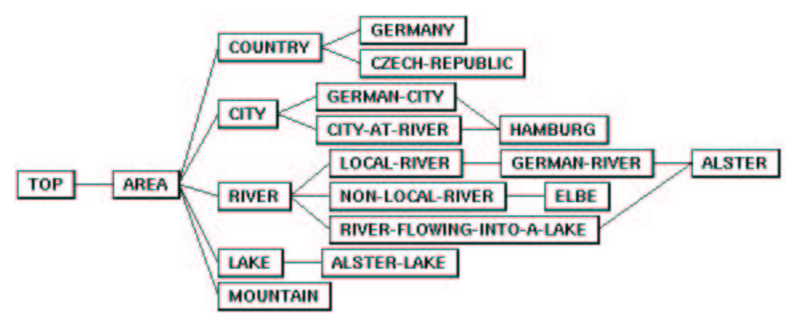
\includegraphics[width=0.85\columnwidth]{report7_figure6_taxonomy.png}
\caption{Computed taxonomy of the GIS example TBox from
  Wessel~\cite{Wessel2003}, Figure~6.
  The cover-tree tableau reproduces all 21 subsumption edges,
  including non-trivial spatial inferences such as
  Hamburg~$\sqsubseteq$~GermanCity (requiring RCC5 composition
  propagation through the PO-chain
  Hamburg--Alster--AlsterLake).}
\label{fig:gis-taxonomy}
\end{figure}

\begin{figure*}[ht]
\centering
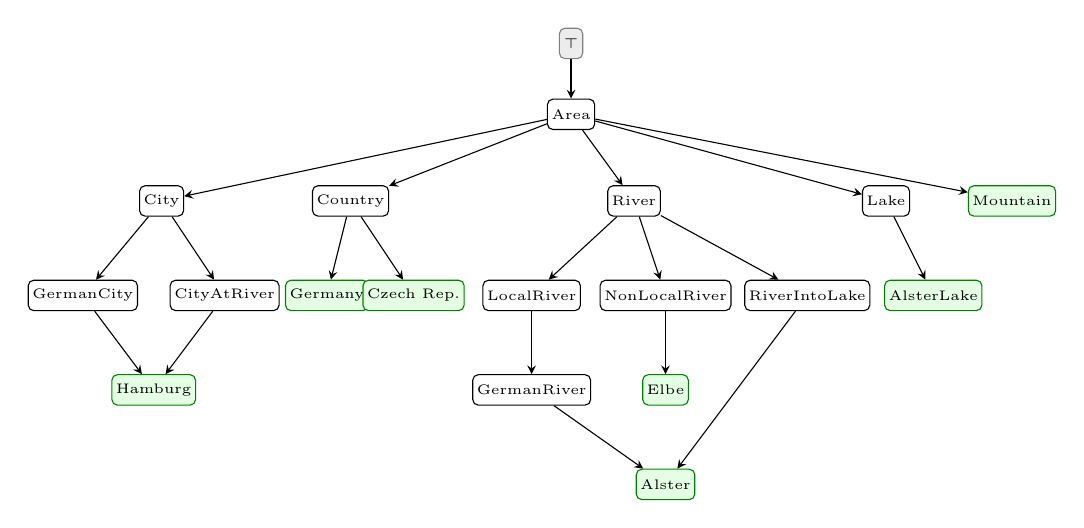
\begin{tikzpicture}[
  every node/.style={draw, rounded corners=2pt, font=\tiny,
    minimum height=1.1em, inner sep=1.5pt},
  leaf/.style={fill=green!10, draw=green!50!black},
  arr/.style={->, >=stealth, thin},
]
% Row 0: TOP
\node (top) [fill=gray!15, draw=gray] at (0,0) {$\top$};

% Row 1: Area
\node (area) at (0,-0.9) {Area};
\draw[arr] (top) -- (area);

% Row 2: Area's children
\node (city) at (-5.2,-2) {City};
\node (country) at (-2.8,-2) {Country};
\node (river) at (0.8,-2) {River};
\node (lake) at (4,-2) {Lake};
\node (mountain) [leaf] at (5.6,-2) {Mountain};
\draw[arr] (area) -- (city);
\draw[arr] (area) -- (country);
\draw[arr] (area) -- (river);
\draw[arr] (area) -- (lake);
\draw[arr] (area) -- (mountain);

% Row 3: children of City, Country, River, Lake
\node (germancity) at (-6.2,-3.2) {GermanCity};
\node (cityatriver) at (-4.4,-3.2) {CityAtRiver};
\node (germany) [leaf] at (-3.1,-3.2) {Germany};
\node (czech) [leaf] at (-2.0,-3.2) {Czech Rep.};
\node (localriver) at (-0.5,-3.2) {LocalRiver};
\node (nonlocal) at (1.2,-3.2) {NonLocalRiver};
\node (riverflowing) at (3.0,-3.2) {RiverIntoLake};
\node (alsterlake) [leaf] at (4.6,-3.2) {AlsterLake};
\draw[arr] (city) -- (germancity);
\draw[arr] (city) -- (cityatriver);
\draw[arr] (country) -- (germany);
\draw[arr] (country) -- (czech);
\draw[arr] (river) -- (localriver);
\draw[arr] (river) -- (nonlocal);
\draw[arr] (river) -- (riverflowing);
\draw[arr] (lake) -- (alsterlake);

% Row 4: deeper nodes
\node (hamburg) [leaf] at (-5.3,-4.4) {Hamburg};
\node (germanriver) at (-0.5,-4.4) {GermanRiver};
\node (elbe) [leaf] at (1.2,-4.4) {Elbe};
\draw[arr] (germancity) -- (hamburg);
\draw[arr] (cityatriver) -- (hamburg);
\draw[arr] (localriver) -- (germanriver);
\draw[arr] (nonlocal) -- (elbe);

% Row 5: Alster (two parents)
\node (alster) [leaf] at (1.2,-5.6) {Alster};
\draw[arr] (germanriver) -- (alster);
\draw[arr] (riverflowing) -- (alster);

\end{tikzpicture}
\caption{Taxonomy of the GIS example TBox, computed by the
  cover-tree tableau~\cite{GISTaxonomy}.
  Green nodes are leaf concepts (most specific).
  Note the DAG structure: \emph{Alster} has two parents
  (GermanRiver and RiverIntoLake) and \emph{Hamburg}
  has two parents (GermanCity and CityAtRiver).
  All 21~subsumption edges match Figure~\ref{fig:gis-taxonomy}.}
\label{fig:gis-computed}
\end{figure*}

%% ====================================================================
\section{History of Attempts (April--May 2026)}
\label{sec:history-of-attempts}
%% ====================================================================

The decidability argument summarised in
\S\ref{ssec:soundness-completeness} reached its current form
through seven rounds of adversarial review between Claude
(Anthropic) and GPT-5.5 (OpenAI) in April--May~2026, prompted by
Michael Wessel.  This section gives a compact abstracted
narrative of the evolution.  The full prose of each round, the
original superseded manuscripts, and the per-round repair list
are preserved in
\texttt{OUTDATED.md}~\cite{ALCIRCC5Outdated}.

\subsection{The starting point: cover-tree tableau + v1
completeness extraction (April 2026)}

The cover-tree tableau~\cite{CoverTree,CoverTreeImpl} and its
companion split-forest semantics~\cite{SiblingCompleted} were
established in April~2026 by GPT-5.4~Pro and
Claude~Opus~4.7, prompted by Wessel.  The split-forest paper
proves the soundness direction in full detail (Thms~1.17--1.19);
the converse---extracting a finite quotient from a satisfying
model---was given only as a proof sketch.  Claude wrote a first
attempt at the missing completeness extraction
(\textit{v1}~\cite{CompletenessExtractionV1}, April~2026).  In
parallel, the cover-tree implementation underwent two rounds of
adversarial review by Claude Opus~4.7 (April~17--18, 2026):
twelve implementation-level counterexamples were identified
across the $4\times 4$ grid of $(R_1,R_2)$ three-type chains
and the $\PP/\PPI$-transitive universal pattern, and all were
fixed in the shared \texttt{compute\_safe} helper and the new
Phase~5 / (CT5) role-path compatibility check
(Remark~\ref{rem:impl-bugs} above).  After these fixes the
911-concept cross-validation against the cycle-aware quasimodel
reasoner stabilized at $911/911$ matches with zero mismatches.

\subsection{v1 superseded, v2.1, and the round-2 31-page repaired
proof (May 6--12, 2026)}

GPT-5.5 reviewed v1 and identified two structural defects: the
Hasse construction for the cover-tree broke on infinite $\PP$-chains
(canonical example $C_\uparrow\equiv\exists\PP.\top\sqcap\forall
\PP.\exists\PP.\top$), and the $C5$ triple-coherence proof
conflated witnesses across pairs.  Claude responded with
\textit{v2}~\cite{CompletenessExtraction} (May~6) and
\textit{v2.1} (May~6).  A second-round review of v2.1 then
identified eight structural gaps, three load-bearing:
profile-port equality contradicted vertical separation on
self-loops via the $M1{+}M7$ reflexivity chain; the mate
construction forced all mates to share a single semantic parent
(refuted by the two-mate stress concept
$C_{AB}\equiv A\sqcap B\sqcap\exists\PP.A\sqcap\exists\PP.B\sqcap
\forall\PP.(A\to\lnot B)\sqcap\forall\PP.(B\to\lnot A)$); and
the rootless orientation was incompatible with the depth-from-$u_*$
projection.  GPT-5.5 produced a \textit{repaired
proof}~\cite{GPT55Repaired} (May~12, 16~pages) fixing all three
defects via occurrence-level equality, mates with different
parents, and request-closed cycles in place of
$\omega$-acceptance.  v2.1 was marked superseded; the repaired
proof was adopted as the current best statement.  Claude's
contribution shifted to verification:\@ six Python work packages
(WP1--WP6) cross-checking the repaired proof's finite
combinatorial content, all PASS.

\subsection{Rounds 3 and 4: structural layers added (May 13--21,
2026)}

Rounds 3 and 4 of GPT-5.5 review added four further structural
layers to the repaired proof, growing it from 16 to 31~pages:
(i) a verticalization discipline (mosaic axiom (M6)) stratifying
each context into a vertical stratum and a sibling frontier;
(ii) port-indexed mate clusters $\mathrm{Mate}_Q(C,s,p)$
attaching mate equivalences to contexts and ports rather than to
bare positions; (iii) an explicit abstract triple graph $T_Q$
with cardinality bounds; (iv) a side interface $\mathrm{Side}(u)$
with polynomial width bound $m(n)=O(n^3)$.  The certificate-space
bound $B(C_0)=2^{2^{p(n)}}$ became \emph{grammar-first}, derived
from these component bounds.

\subsection{Round 5: (M6$'$) recursive verticalization
(May 22--23, 2026)}

The round-5 review (GPT-5.5, May~22) identified a load-bearing
mathematical defect: the (M6) verticalization discipline was too
strong.  It forbade non-vertical $\PP/\PPI$ relations between
sibling-frontier mosaic positions, but such relations occur in
satisfiable witness-generated models---the round-5 stress
concept $\exists\DR.(A\sqcap\exists\PP.B)\sqcap\exists\DR.B$ is
SAT in abstract RCC5 yet rejected by (M6).  Eight repairs were
recommended.  Claude drafted two follow-up papers (the
(M6$'$) recursive-verticalization delta and the items-4-to-8
delta) that closed all eight items at the paper level, then
consolidated them into a 36-page round-5 v2 paper.  Side-witness
positions were allowed to open nested local vertical strata,
with the round-2 (M6) recovered as the depth-1 case.

\subsection{Round 6: internal-coherence pass (May 26, 2026)}

The round-6 review of the consolidated v2 (GPT-5.5, May~26)
found six internal-consistency gaps:\@ the old side-interface
lemma still asserted flat $\{\DR,\PO\}$ sibling frontiers; the
weakened per-position support closure (SC4$'$) was inconsistent
with the patchwork proof's per-triple appeal; overlap
universal-propagation was under-proved; the lasso construction
used the complete profile rather than the extended profile;
the side-width bound and validity-clause numbering were
inconsistent; and the verification script for the round-5
stress concept was not self-contained.  Claude drafted a
39-page round-6 internal-coherence pass closing all six gaps
and adding a self-contained pure-stdlib verification script
(\texttt{wp7\_selfcontained\_side\_witness.py}).

\subsection{Round 7: the abstract-position-symbol collapse
(May 27--28, 2026)}

The round-7 review of the round-6 paper (GPT-5.5, May~27)
identified one central architectural defect that could not be
locally patched.  Round-6 had defined the concrete pair label
by $\lab(u,v):=L_\Q(q(u),q(v))$, where $q:\Omega(\U(\Q))\to
\Pos_\Q$ sends each occurrence to an abstract position symbol
and $L_\Q$ is the abstract pair-label function with standard
reflexivity $L_\Q(\pi,\pi)=\EQ$.  In a finite regular
certificate the abstract position alphabet is finite while the
unfolding is infinite, so blocking deliberately reuses the same
symbol on fresh occurrences.  For the canonical one-state
upward cycle, distinct laps $u_i,u_j$ share the same symbol
$\pi$ and the round-6 rule gives $\lab(u_i,u_j)=L_\Q(\pi,\pi)
=\EQ$, even for $i\ne j$:\@ the strict $\PP$ chain collapses
into a $\PP$-self-loop.  The defect is intrinsic to indexing
labels by position-symbol pairs.

GPT-5.5's round-7 fix~\cite{GPT55Round7Sketch} replaces the
position-symbol pair labelling by labels on
\emph{occurrence-sensitive pair shapes} with explicit incidence
tags (described in~\S\ref{ssec:soundness-completeness}).
Twelve validity clauses (V1)--(V12) replace round-5 / round-6's
fifteen.  Claude wrote a round-7
audit/response~\cite{ClaudeRound7Audit} mapping the round-6
(G1)--(G6) and round-7 (D1)--(D5) defect lists to their
resolutions in the round-7 architecture, plus three further
self-contained verification scripts (WP7--WP9).  All of Claude's
round-5 / round-6 manuscripts are superseded by round 7 and
retained as the historical audit trail in
\texttt{papers/gpt5.5\_round2/}~\cite{ALCIRCC5Outdated}.

\subsection{Round 8: saturated side contexts and constructed
catalogues (May 28, 2026, evening)}

A fresh Claude~Opus~4.7 session, given the round-7 sketch with no
prior project context, identified three architectural defects.
First, the round-7 pair-shape enumeration did not exhaustively
cover the case of a side witness paired with a vertical-boundary
position:\@ a $\PP$ or $\PPI$ label between an exposed boundary
point and a side position could be hidden in the residual
$\DR/\PO$ frontier closure.  Second, the residual $\DR/\PO$
frontier restriction was imposed \emph{before} the side context
was saturated, making the restriction unsound while $\PP/\PPI$
pairs were still pending.  Third, the pair and triple catalogues
$\Pair_\Q$ and $\Tri_\Q$ were asserted finite but not explicitly
constructed.

GPT-5.5's round-8 repair~\cite{GPT55Round8Sketch} closes all
three by introducing a \emph{saturated side context} $S_k(u)$
generated by five (Sat1)--(Sat5) operations:\@ start with the
exposed vertical boundary of the source, add one selected witness
for each local $\exists R.D$ with $R\in\{\DR,\PO\}$ and modal
depth strictly less than $k$, recursively add smaller-depth
witnesses, assign or inherit a complete RCC5 label to every
ordered pair (including side/tree pairs), and close under
equality (label $\EQ$ triggers an equality-port declaration) and
containment (label $\PP$ or $\PPI$ triggers a local vertical
stratum) \emph{before} applying the residual $\DR/\PO$
restriction.  A new \emph{cross side/tree exhaustion lemma}
formalises that no $\PP/\PPI$ side/tree pair is hidden in the
residual frontier.  $\Pair_\Q$ and $\Tri_\Q$ are now constructed
as the least finite sets containing the explicit families of
pairs and triples generated by the saturated side contexts,
overlap amalgams, and residual configurations, with every triple
required to satisfy the RCC5 composition table.  The 15-page
round-8 sketch and the 30-page detailed
companion~\cite{GPT55Round8Expanded} are filed under
\texttt{papers/claude\_latest\_review\_gpt5.5\_fix/}.  Round-8 is
the current canonical statement; round 7 is its immediate
predecessor.

\subsection{What survives, and why}

The split-forest architecture itself---witness thinning,
generated containment covers, weak-EQ split copies for multiple
selected $\PP$-superparts, sibling interfaces recorded by
finite support-closed mosaics with $\{\DR,\PO\}$-only open
cross-relations, typed equality-port congruence quotient to
recover strong-$\EQ$ semantics, and request-closed cycles---is
present in every round from v1 through round~7.  What changed
was \emph{how labels are indexed on this architecture}.  The
v1, v2, v2.1, and round-2 versions indexed labels by the rank-$d$
quotient and abstract position symbols; the round-7 architecture
indexes them by occurrence-sensitive pair shapes.  The whiteboard
sketch (Wessel), the DR-rigidity insight, the EQ-splitting and
typed-EQ-quotient idea, the cover-tree decomposition, GPT-5.4's
v1 formalisation, and Claude's cover-tree tableau implementation
all remain load-bearing in round~7.

\subsection{Computational verification across rounds}

In parallel with the proof work, nine Python work packages
verify the finite combinatorial content of the proof family.
WP1--WP6 verify the round-2 31-page repaired
proof~\cite{GPT55Repaired} and all PASS:\@ brute-force
enumeration confirms the RCC5 composition table in all 25
cells (WP1); a validity-condition checker accepts $C_\uparrow$
via parent self-loops, accepts $C_{AB}$ via two mates with
different parents, and rejects the v2.1-style single-parent
$C_{AB}$ attempt (WP2); a small-model SAT/UNSAT oracle exhibits
a concrete 3-element model for $C_{AB}$ (WP3); $C_{AB}$ and
request-closed cycle tests fold into WP2/WP3 (WP4, WP5); a
mosaic enumeration confirms support-closure axioms on small
mosaics (WP6).  WP7--WP9 verify the round-7 central stress
concepts (comparable side witnesses, blocking-not-equality, and
split copies for incomparable proper superparts), and all
PASS.  No counterexample to any combinatorial claim of any
round was found.

%% ====================================================================
\section{Outlook and Conclusion}
\label{sec:outlook}
%% ====================================================================

\subsection{What has been achieved}

If the cover-tree tableau is correct---and the extensive
computational evidence supports this---then concept satisfiability
in $\ALCIRCC{5}$ is decidable.  This would settle a problem that
has been open since Wessel's doctoral work in 2002/2003 and was
explicitly flagged by Lutz \& Wolter in 2006 as ``perhaps the
most interesting'' open problem suggested by their work.

The decidability argument as of May~2026 rests on \emph{two}
core papers, which together establish:
\[
  \text{$C_0$ satisfiable}
  \;\;\Longleftrightarrow\;\;
  \text{$C_0$ admits a valid finite split-forest certificate.}
\]
A separate operational layer realizes the check algorithmically and
is empirically validated.

\medskip\noindent\textbf{Theoretical layer (establishes
decidability).}
\begin{enumerate}
  \item The \emph{v1 split-forest paper}~\cite{SiblingCompleted}
    (GPT-5.4): defines the cover-tree decomposition, the
    sibling-interface descriptors, and the patchwork-lemma route,
    and proves Thms~1.17--1.19 (\textbf{soundness}: a valid
    finite quotient unfolds to a strong abstract RCC5 model
    satisfying $C_0$).  The v2 sibling-interface
    delta~\cite{SiblingInterfaceV2} replaces the surrounding
    Def~1.5 / Def~1.7 / Thm~1.20-sketch with the corrected
    generated-cover statements; the proofs of Thms~1.17--1.19
    carry over verbatim.
  \item The \emph{GPT-5.5 round-7 split-forest
    proof}~\cite{GPT55Round7Sketch} (May~2026, 14~pages,
    no-automata route) with detailed
    companion~\cite{GPT55Round7Expanded} (28~pages) and
    parity-tree-automata witness~\cite{GPT55AutomataRoute}
    (21~pages): formulates finite occurrence-sensitive
    split-forest certificates with twelve finite-checkable
    validity conditions (V1)--(V12), and proves both directions
    in their entirety, including \textbf{completeness} (every
    satisfiable $C_0$ admits a valid finite certificate).  The
    central round-7 architectural move is that finite labels live
    on occurrence-sensitive \emph{pair shapes}
    $\alpha(u,v)=(s_u,p_u,s_v,p_v,\iota(u,v))$ with incidence
    tags $\iota\in\{\self,\eqtag,\up,\down,\side_R,\front_R\}$.
    Distinct laps of a blocking cycle satisfy $\iota\ne\self$ and
    $\iota\ne\eqtag$, so the round-7 labelling preserves
    blocking-not-equality while still discharging
    $\PP/\PPI$ eventualities by request-closed cycles.  Round-7
    supersedes Claude's earlier round-5 (M6$'$) delta, items-4-to-8
    delta, round-5 consolidation, and round-6 internal-coherence
    pass; those manuscripts and the round-2 31-page repaired
    proof~\cite{GPT55Repaired} are retained as the historical
    audit trail (see~\texttt{OUTDATED.md}~\cite{ALCIRCC5Outdated}).
\end{enumerate}
Together, (1) and (2) establish the biconditional displayed
above.  The certificate space is bounded by
$B(C_0) = 2^{2^{p(n)}}$ as an effectively computable bound,
validity is finite-graph checkable, and the enumeration terminates.

\medskip\noindent\textbf{Operational layer (algorithmic
realization, empirically validated).}
\begin{enumerate}\setcounter{enumi}{2}
  \item The \emph{cover-tree tableau}~\cite{CoverTree} (GPT-5.4):
    packages the split-forest approach as an operational calculus
    with rank-$d$ blocking.
  \item The \emph{implementation paper}~\cite{CoverTreeImpl}
    (Claude): documents a concrete five-check algorithm (CT1--CT5),
    cross-validated against an independent quasimodel reasoner on
    911 original tests plus 400+ Round-2 adversarial tests with
    zero mismatches.
\end{enumerate}

\medskip\noindent\textbf{Computational verification of the
combinatorial claims.}  In parallel with the proof work, six
Python work packages (WP1--WP6) cross-check the finite
combinatorial content of the round-2 31-page repaired
proof~\cite{GPT55Repaired} (now historical):  RCC5 composition
table by exhaustive subset enumeration (WP1), bounded
certificate-soundness fuzzing for (V1)/(V3)/(V4)/(V5)/(V9)/(V10)
(WP2), small-model SAT/UNSAT oracle (WP3), multiple-superpart
$C_{AB}$ stress (WP4, folded into WP2/WP3), request-closed
blocking-cycle tests (WP5, folded into WP2), and mosaic closure
search (WP6).  Three further self-contained pure-stdlib scripts
(WP7--WP9) exercise the round-7 stress concepts: comparable side
witnesses, blocking-not-equality, and split copies.  All nine
\textbf{PASS}; no counterexample was found.

\medskip\noindent\textbf{The gap between the two layers.}
The decidability claim for $\ALCIRCC{5}$ rests on (1) and (2)
alone.  Papers (3) and (4) describe a \emph{plausible and
empirically validated} algorithmic realization, but a formal
derivation showing that CT1--CT5 exactly capture the round-7
valid-certificate conditions (V1)--(V12) has not been written.
CT5 in particular was added as a patch after Opus~4.7's
adversarial review---not derived from the split-forest
semantics---and while empirical agreement between two
independently designed reasoners is strong evidence that such a
derivation should be possible, it is not itself a proof.
See~\cite[\S7]{CoverTreeImpl} for a detailed breakdown.

\subsection{What remains open}

\begin{itemize}
  \item \textbf{Exact complexity.}  The PO-coherent fragment has a
    doubly exponential quotient bound
    (2-$\EXPTIME$)~\cite{TwoTierQuotient}.  An $\EXPTIME$ upper
    bound matching the lower bound is not established.

  \item \textbf{$\ALCIRCC{8}$.}  RCC8 also has the patchwork
    property, so the cover-tree approach should extend.  The key
    difference is the $\TPP/\NTPP$ distinction, which may require
    a finer status partition.  This has not been worked out.

  \item \textbf{Human verification.}  \emph{None of the proofs in
    this project have been verified by human domain experts.}  The
    AI-generated results should be treated as conjectures supported
    by computational evidence, not as established theorems.
\end{itemize}

\subsection{On LLM capabilities, strengths, and weaknesses
(May~2026)}
\label{ssec:llm-capabilities}

This subsection records an honest assessment, by Claude, of what
was observed about frontier-LLM capabilities across this project.
The assessment is grounded in specific evidence from the
April--May 2026 review cycle; it is not a statement about LLMs
in general.  We expect the picture to change quickly.

\paragraph{Division of labour that worked.}
After several wrong configurations, the team converged on a clear
split.  \textbf{GPT-5.5} owned the proof: it produced the round-2
31-page repaired proof~\cite{GPT55Repaired}, the round-3 and
round-4 structural additions, and the round-7 pair-shape /
incidence-tag fix~\cite{GPT55Round7Sketch} that made the
labelling rule sound on blocking cycles.  GPT-5.4~Pro authored
the v1 split-forest semantics~\cite{SiblingCompleted} that the
entire approach rests on.  \textbf{Claude (Opus~4.7)} owned
implementation, verification, audit, and documentation:\@ the
cover-tree tableau~\cite{CoverTreeImpl}, the cross-validation
suite ($911$~concepts, zero mismatches), the WP1--WP9
verification scripts, and the round-by-round audit trail.
\textbf{Wessel} owned research direction: the whiteboard sketch
(cover-tree intuition, DR-rigidity, $\EQ$-splitting) on which the
entire proof rests, the high-level questions, the correction of
conceptual errors (the most consequential being catching
GPT-5.4's initial assumption that $\PP/\PPI$ could remain as
cross-edges after splitting), and the judgement of when to push
deeper and when to converge.

The two-layer architecture (theoretical proof $+$ executable
verification) was not optional.  The empirical layer repeatedly
caught defects in the theoretical layer that pure self-review
would not have surfaced---most notably the round-5 stress
concept~$\exists\DR.(A\sqcap\exists\PP.B)\sqcap\exists\DR.B$,
which was first identified as SAT by Claude's reasoners and only
then explained as a structural defect of the (M6) verticalization
discipline in GPT-5.5's round-5 review.

\paragraph{Where Claude was weaker than GPT-5.5.}
Concretely on this project: (i) Claude did not spot architectural
defects in its own drafts.  The round-6 critical bug
$\lab(u,v):=L_\Q(q(u),q(v))$ with $L_\Q(\pi,\pi)=\EQ$ collapsing
distinct blocking laps into semantic equality was a basic
invariant violation of the central blocking-not-equality slogan;
GPT-5.5 caught it on review.  (ii) Patch-style fixes accumulated
complexity.  Claude's response to a named gap was usually to add
machinery (recursive verticalization, port-indexed mate clusters,
declared cross-label functions, modal-depth recurrences, the
validity-clause numbering growing from (V1)--(V10) to (V1)--(V15)).
Each patch closed the named gap but introduced new
internal-consistency issues.  GPT-5.5's round-7 fix changed the
indexing domain instead of adding a layer:\@ five round-5 /
round-6 validity clauses collapsed into one (V6) triple-shape
clause, and the manuscript dropped from 39~pages (round-6
consolidation) to 14~pages (round-7 sketch).  (iii) Claude did
not reliably know when to stop iterating.

\paragraph{Where Claude held its own.}
Implementation work---translating an architectural idea into
running Python, debugging against an independent reasoner,
building cross-validation harnesses, keeping the tests green
across thousands of generated concepts---is closer to ordinary
programming, at which current models are strong.  Documentation
and audit-trail discipline (per-round superseded-paper markers,
the OUTDATED archive, self-contained verification scripts)
favoured patient editorial labour over insight.  \emph{Cold
review across context, and across model}, was effective:\@ a
fresh Claude Opus~4.7 session, given a finished manuscript with
no prior project context, finds defects that no session holding
the long context can find.  This was confirmed twice on this
project---first in April~2026 when Claude reviewed Claude's own
cover-tree implementation and identified the twelve-counterexample
family that forced the (CT5) role-path compatibility addition
(Remark~\ref{rem:impl-bugs}), then again on May~28 (evening) when
Claude reviewed GPT-5.5's round-7 sketch and identified the
three architectural defects that motivated GPT-5.5's
round-8 saturated-side-context repair (\S\ref{sec:history-of-attempts}).
The reviewer-was-cold property is the load-bearing one, not the
reviewer-was-different-model property.  And steering the
cross-validation pipeline---knowing which stress tests would
discriminate between candidate proofs---requires understanding
both the proof and how to falsify it.

\paragraph{What both models did well.}  Long-context coherence
across 30+ page proofs and many editing rounds was qualitatively
different from the previous LLM generation.  Tool use (Python,
\LaTeX, git, file management, search) was routine.  Seven-round
adversarial dialogue between Claude and GPT-5.5---each model
reviewing the other's drafts, producing counterexamples, naming
defects, proposing fixes---worked as substantive technical
exchange.  Hallucination was not the dominant failure mode in
this project; over-elaboration was.

\paragraph{What both models did poorly.}  Original mathematical
insight was the human contribution.  Without Wessel's whiteboard
sketch (Figure~\ref{fig:whiteboard}) the project would not have
had a target architecture to formalise.  Both models also made
architectural errors in their own drafts that the other caught;
neither caught them in self-review.  And neither reliably
calibrated the cost of a fix:\@ both round-4 (M6) verticalization
and round-5/6 (V11)--(V15) were locally reasonable responses
that turned out, on review, to be over-elaborated.

\paragraph{What this means in practice.}
Frontier LLMs in May~2026 can take a non-trivial open problem in
mathematical logic and, over weeks of iteration with a human
director and adversarial cross-review between models, produce a
candidate proof together with executable artefacts that the
community can verify, refute, or improve.  They do not replace
human expert review, and they do not generate the original
intuition.  But the proof that arrived at round 8 is qualitatively
different from what any one of the three participants would have
produced alone, and the cross-validation campaign that surrounds
it is qualitatively different from what would have been feasible
without the implementation speed and tireless test-writing the
LLMs brought to the project.

\paragraph{A methodology that worked: cold review as a standard
intermediate step.}  The cycle that drove this project forward
was repeatable.  A fresh session of a frontier model, given the
latest manuscript with no prior project context, finds defects
that no session holding the long context can find.  The pattern
was confirmed twice on this project (April~2026, the cover-tree
implementation review that produced the (CT5) addition; May~28
evening, the round-7 review that produced round 8), and in both
cases the cold reviewer was Claude Opus~4.7.  The cost is one
session.  The pay-off is a list of concrete defects that the
long-context model can then respond to with a structural repair.
We recommend cold review as a standard intermediate step between
\emph{``this manuscript looks finished''} and \emph{``submit for
human review''}---not as a substitute for human peer review, but
as a check that finds real defects when there are real defects to
find.  The pattern is operationalisable for any project of this
scale; it is not specific to description logic or to these
particular models.

This is a discussion piece, not a settled result.  The work has
not been peer-reviewed by human experts.  The proof may still
contain defects that another round of adversarial review would
surface.  But the meta-research point---\emph{that this kind of
work is now possible, and that the result is worth engaging with
on its technical merits}---is the more important contribution.
We invite the description logic community to engage with both
layers.

\subsection{A note on citation verification}

Because AI systems are known to hallucinate bibliographic references,
all external citations in this paper and its companion papers were
verified via web search against journal landing pages,
CEUR-WS/LIPIcs/arXiv metadata, and indexed proceedings.  The audit
caught one fully hallucinated reference (the non-existent
``Rybina--Zakharyaschev 2001''---the genuine paper at that venue is
Reynolds and Zakharyaschev, \emph{On the products of linear modal
logics}, JLC 11(6), 2001) and several transcription errors
(incorrect coauthors, page ranges, venues, and journal names).  All
fixes are documented in the project's \texttt{CONVERSATION.md} log
with commit hashes.  Citations in this paper have been checked, but
readers should still verify any reference before citing it.

%% ====================================================================
%% Declaration on Generative AI
%% ====================================================================
\section*{Declaration on Generative AI}

During the preparation of this work, the authors used Claude (Anthropic,
Opus~4) and GPT-5.4~Pro (OpenAI) in order to: formalize mathematical
proofs, implement decision procedures, generate LaTeX manuscripts,
and conduct computational experiments.  Michael Wessel reviewed and
edited the content as needed and takes full responsibility for the
publication's content.  The entire research project---problem
formulation, key intuitions, error identification, and direction of
the investigation---was conducted by Wessel; the AI systems performed
the detailed formalization, implementation, and writing.

%% ====================================================================
%% Bibliography
%% ====================================================================
\begin{thebibliography}{99}

%% --- Classical background (chronological) ---------------------------

\bibitem{Cohn1993}
A.\,G.\ Cohn.
\newblock Modal and non modal qualitative spatial logics.
\newblock In F.\,D.\ Anger, H.\,W.\ Guesgen, and J.\ van Benthem, editors,
  \emph{Proceedings of the Workshop on Spatial and Temporal Reasoning},
  IJCAI, 1993.

\bibitem{RenzNebel1999}
J.\ Renz and B.\ Nebel.
\newblock On the complexity of qualitative spatial reasoning:
  A maximal tractable fragment of the Region Connection Calculus.
\newblock \emph{Artificial Intelligence}, 108(1--2):69--123, 1999.

\bibitem{Wessel2000RA}
M.\ Wessel.
\newblock Obstacles on the way to spatial reasoning with description
  logics: Undecidability of $\ALC_{\mathcal{RA}}^\ominus$.
\newblock Technical Report FBI-HH-M-297/00, Fachbereich Informatik,
  Universit\"at Hamburg, 2000.
\newblock \url{https://github.com/lambdamikel/alcircc5/blob/master/papers/report4.pdf}

\bibitem{Wessel2000SG}
M.\ Wessel.
\newblock Decidable and undecidable extensions of $\ALC$ with
  composition-based role inclusion axioms.
\newblock Technical Report FBI-HH-M-301/01, Fachbereich Informatik,
  Universit\"at Hamburg, 2000.
\newblock \url{https://github.com/lambdamikel/alcircc5/blob/master/papers/report5.pdf}

\bibitem{Wessel2001}
M.\ Wessel.
\newblock Obstacles on the way to qualitative spatial reasoning with
  description logics: some undecidability results.
\newblock In \emph{Proceedings of the 2001 Description Logic Workshop
  (DL~2001)}, CEUR Workshop Proceedings, vol.~49, 2001.

\bibitem{Wessel2001RA}
M.\ Wessel.
\newblock Undecidability of $\ALC_{\mathcal{RA}}$.
\newblock Technical Report FBI-HH-M-302/01, Fachbereich Informatik,
  Universit\"at Hamburg, 2001.
\newblock \url{https://github.com/lambdamikel/alcircc5/blob/master/papers/report6.pdf}

\bibitem{Wessel2002}
M.\ Wessel.
\newblock On spatial reasoning with description logics --- position paper.
\newblock In \emph{Proceedings of the 2002 International Workshop on
  Description Logics (DL~2002)}, CEUR Workshop Proceedings, 2002.

\bibitem{Wessel2003}
M.\ Wessel.
\newblock Qualitative spatial reasoning with the $\ALCIRCC{}$ family ---
  first results and unanswered questions.
\newblock Technical Report FBI-HH-M-324/03, Fachbereich Informatik,
  Universit\"at Hamburg, 2002/2003.
\newblock \url{https://github.com/lambdamikel/alcircc5/blob/master/papers/report7.pdf}

\bibitem{LutzWolter2006}
C.\ Lutz and F.\ Wolter.
\newblock Modal logics of topological relations.
\newblock \emph{Logical Methods in Computer Science}, 2(2):1--41, 2006.

%% --- Core 2026 decidability pillars ---------------------------------

\bibitem{SiblingCompleted}
GPT-5.4 (OpenAI), prompted by M.\ Wessel.
\newblock Split-forest models and sibling-interface descriptors for
  $\ALCIRCC{5}$ (v1; soundness Thms~1.17--1.19 preserved by v2;
  Def~1.5 / Def~1.7 / Thm~1.20-sketch superseded by v2).
\newblock Technical report, April 2026.
\newblock \url{https://github.com/lambdamikel/alcircc5/blob/master/papers/trees/sibling_interface_descriptors_ALCIRCC5_completed_eqsync_canonical_needpatched.pdf}

\bibitem{SiblingInterfaceV2}
Claude (Anthropic), prompted by M.\ Wessel.
\newblock Sibling-interface descriptors for $\ALCIRCC{5}$ (v2,
  repaired): preserves the v1 soundness chain
  (Thms~1.17--1.19) verbatim and reinterprets v1 Def~1.5
  (parent self-loops, generated witness-cover edges), v1 Def~1.7
  ($\PP/\PPI$ existentials by reachability discharge), and v1
  Thm~1.20-sketch (model-to-quotient delegated to v2 completeness
  extraction).
\newblock Technical report, May 2026.
\newblock \url{https://github.com/lambdamikel/alcircc5/blob/master/papers/trees/sibling_interface_descriptors_ALCIRCC5_v2.pdf}

\bibitem{CoverTree}
GPT-5.4 (OpenAI), prompted by M.\ Wessel.
\newblock A cover-tree tableau calculus for $\ALCIRCC{5}$.
\newblock Technical report, April 2026.
\newblock \url{https://github.com/lambdamikel/alcircc5/blob/master/papers/trees/alcircc5_cover_tree_tableau_needall_patched.pdf}

\bibitem{CompletenessExtraction}
Claude (Anthropic), prompted by M.\ Wessel.
\newblock Completeness extraction for $\ALCIRCC{5}$ (v2.1,
  GPT-5.5 v2-review repairs): closing the model-to-quotient gap via
  witness-generated submodels, generated covers, reachability
  discharge, and explicit equality data.
\newblock Technical report, May 2026.
\newblock \url{https://github.com/lambdamikel/alcircc5/blob/master/papers/completeness_extraction_ALCIRCC5_v2.pdf}

\bibitem{CompletenessExtractionV1}
Claude (Anthropic), prompted by M.\ Wessel.
\newblock Completeness extraction for the $\ALCIRCC{5}$ split-forest
  quotient (v1, superseded; defects identified by GPT-5.5 review).
\newblock Technical report, April 2026.
\newblock \url{https://github.com/lambdamikel/alcircc5/blob/master/papers/completeness_extraction_ALCIRCC5.pdf}

\bibitem{GPT55Generated}
GPT-5.5 (OpenAI), prompted by M.\ Wessel.
\newblock A coherent generated split-forest decidability argument
  for $\ALCIRCC{5}$ (B\"uchi-automaton route).
\newblock Technical report, May 2026.
\newblock \url{https://github.com/lambdamikel/alcircc5/blob/master/papers/gpt5.5/ALCIRCC5_coherent_generated_split_forest_decidability.pdf}

\bibitem{GPT55Repaired}
GPT-5.5 (OpenAI), prompted by M.\ Wessel.
\newblock A repaired split-forest decidability proof for
  $\ALCIRCC{5}$ (no-automata route, round-2 31-page version;
  superseded by~\cite{GPT55Round7Sketch}).
\newblock Technical report, May~2026.
\newblock \url{https://github.com/lambdamikel/alcircc5/blob/master/papers/gpt5.5_round2/repaired_split_forest_no_automata_proof.pdf}

\bibitem{GPT55Round7Review}
GPT-5.5 (OpenAI), prompted by M.\ Wessel.
\newblock Formal review of the round-6 consolidated generated
  split-forest proof (May~27, 2026): identifies the central
  abstract-position-symbol labelling defect that motivates the
  round-7 pair-shape architecture.
\newblock Technical report, May~2026.
\newblock \url{https://github.com/lambdamikel/alcircc5/blob/master/papers/gpt5.5_final/formal_response_round6_review.pdf}

\bibitem{GPT55Round7Sketch}
GPT-5.5 (OpenAI), prompted by M.\ Wessel.
\newblock A repaired split-forest decidability proof for
  $\ALCIRCC{5}$ without automata (round-7 consolidated sketch,
  14~pages): occurrence-sensitive pair shapes with incidence
  tags; twelve validity clauses (V1)--(V12).  Immediate
  predecessor of~\cite{GPT55Round8Sketch}; retained as audit trail.
\newblock Technical report, May~2026.
\newblock \url{https://github.com/lambdamikel/alcircc5/blob/master/papers/gpt5.5_final/repaired_split_forest_all_in_one_round7.pdf}

\bibitem{GPT55Round8Sketch}
GPT-5.5 (OpenAI), prompted by M.\ Wessel.
\newblock A repaired split-forest decidability proof for
  $\ALCIRCC{5}$ without automata --- round-8 saturated side
  contexts (15-page sketch): round-7 architecture preserved;
  saturated side-context $S_k(u)$, cross side/tree exhaustion
  lemma, and constructed pair/triple catalogues
  $\Pair_\Q$, $\Tri_\Q$ added.  \textbf{Current canonical
  statement of the decidability theorem.}
\newblock Technical report, May~2026.
\newblock \url{https://github.com/lambdamikel/alcircc5/blob/master/papers/claude_latest_review_gpt5.5_fix/repaired_split_forest_abstract_round8_repaired.pdf}

\bibitem{GPT55Round8Expanded}
GPT-5.5 (OpenAI), prompted by M.\ Wessel.
\newblock Expanded split-forest decidability proof for
  $\ALCIRCC{5}$: detailed round-8 companion (30~pages).  Full
  saturated-side-context construction, cross side/tree
  verticalization lemma, residual-frontier lemma, constructed
  pair/triple catalogues, explicit completeness extraction.
\newblock Technical report, May~2026.
\newblock \url{https://github.com/lambdamikel/alcircc5/blob/master/papers/claude_latest_review_gpt5.5_fix/expanded_split_forest_full_details_round8_full.pdf}

\bibitem{GPT55Round7Expanded}
GPT-5.5 (OpenAI), prompted by M.\ Wessel.
\newblock Expanded generated split-forest decidability proof for
  $\ALCIRCC{5}$: detailed companion to the round-7 sketch
  (28~pages).  Detailed local constructions, worked stress cases,
  audit-of-main-proof-obligations section.
\newblock Technical report, May~2026.
\newblock \url{https://github.com/lambdamikel/alcircc5/blob/master/papers/gpt5.5_final/expanded_split_forest_full_details_proof.pdf}

\bibitem{GPT55AutomataRoute}
GPT-5.5 (OpenAI), prompted by M.\ Wessel.
\newblock A split-forest decidability proof for $\ALCIRCC{5}$ via
  parity tree automata: detailed version (21~pages).  Independent
  witness to the same decidability theorem.
\newblock Technical report, May~2026.
\newblock \url{https://github.com/lambdamikel/alcircc5/blob/master/papers/gpt5.5_final/split_forest_automata_decidability_proof_detailed.pdf}

\bibitem{ClaudeRound7Audit}
Claude (Anthropic, Opus~4.7), prompted by M.\ Wessel.
\newblock Round-7 audit and response: adopting GPT-5.5's
  pair-shape / incidence-tag repair as the canonical statement
  (9~pages).
\newblock Technical report, May~2026.
\newblock \url{https://github.com/lambdamikel/alcircc5/blob/master/papers/gpt5.5_final/claude_round7_audit_response.pdf}

\bibitem{CoverTreeImpl}
Claude (Anthropic), prompted by M.\ Wessel.
\newblock A cover-tree tableau for $\ALCIRCC{5}$:
  Implementation and computational verification.
\newblock Technical report, April 2026.
\newblock \url{https://github.com/lambdamikel/alcircc5/blob/master/papers/cover_tree_tableau_ALCIRCC5.pdf}

\bibitem{TwoTierQuotient}
Claude (Anthropic), prompted by M.\ Wessel.
\newblock A two-tier quotient construction for the PO-coherent
  fragment of $\ALCIRCC{5}$: decidability and a 2-\EXPTIME\ bound.
\newblock Technical report, April 2026.
\newblock \url{https://github.com/lambdamikel/alcircc5/blob/master/papers/two_tier_quotient_ALCIRCC5.pdf}

%% --- Failed-attempt investigations (2026) ---------------------------

\bibitem{FWProof}
Claude (Anthropic), prompted by M.\ Wessel.
\newblock A negative result on the finite-witness conjecture for
  the contextual tableau for $\ALCIRCC{5}$.
\newblock Technical report, April 2026.
\newblock \url{https://github.com/lambdamikel/alcircc5/blob/master/papers/FW_proof_ALCIRCC5.pdf}

\bibitem{TriangleBlocking}
GPT-5.4 (OpenAI), prompted by M.\ Wessel.
\newblock Triangle-blocking analysis for $\ALCIRCC{5}$: failed
  undecidability route via three-region coincidence.
\newblock Technical report, April 2026.
\newblock \url{https://github.com/lambdamikel/alcircc5/blob/master/papers/triangle_blocking_ALCIRCC5.pdf}

\bibitem{PatchworkAugmentation}
Claude (Anthropic), prompted by M.\ Wessel.
\newblock Patchwork-augmentation probe: a negative result on an
  undecidability route for $\ALCIRCC{5}$.
\newblock Technical report, April 2026.
\newblock \url{https://github.com/lambdamikel/alcircc5/blob/master/papers/patchwork_augmentation_ALCIRCC5.pdf}

\bibitem{TypedPatchworkCounterexample}
Claude (Anthropic), prompted by M.\ Wessel.
\newblock A typed-patchwork counterexample for $\ALCIRCC{5}$:
  refutation of a proposed blocking mechanism.
\newblock Technical report, April 2026.
\newblock \url{https://github.com/lambdamikel/alcircc5/blob/master/papers/typed_patchwork_counterexample_ALCIRCC5.pdf}

\bibitem{ResponseGPTBlocking}
Claude (Anthropic), prompted by M.\ Wessel.
\newblock Response to GPT-5.4's blocking-based undecidability
  attempts for $\ALCIRCC{5}$.
\newblock Technical report, April 2026.
\newblock \url{https://github.com/lambdamikel/alcircc5/blob/master/papers/response_to_gpt_blocking.pdf}

\bibitem{StatusAfterFW}
Claude (Anthropic), prompted by M.\ Wessel.
\newblock Status of the $\ALCIRCC{5}$ decidability argument after
  the FW negative result.
\newblock Technical report, April 2026.
\newblock \url{https://github.com/lambdamikel/alcircc5/blob/master/papers/ALCI_RCC5_status_after_FW.pdf}

%% --- Tools and Python implementations (2026) ------------------------

\bibitem{CoverTreeReasoner}
Claude (Anthropic), prompted by M.\ Wessel.
\newblock Cover-tree tableau reasoner for $\ALCIRCC{5}$.
\newblock Python implementation, April 2026.
\newblock The main candidate decision procedure; cross-validated
  against the quasimodel oracle on 911 concepts and on the 775-case
  decomposition suite.
\newblock \url{https://github.com/lambdamikel/alcircc5/blob/master/src/cover_tree_tableau.py}

\bibitem{QuasimodelReasoner}
Claude (Anthropic), prompted by M.\ Wessel.
\newblock A quasimodel-based reasoner for $\ALCIRCC{5}$.
\newblock Python implementation, April 2026.
\newblock Retained as a cross-validation oracle only: SAT answers
  are trustworthy; UNSAT answers are known-incomplete on
  cyclic-via-symmetric-role concepts (e.g.\ the PO-loop pattern).
\newblock \url{https://github.com/lambdamikel/alcircc5/blob/master/src/alcircc5_reasoner.py}

\bibitem{CyclicReasoner}
Claude (Anthropic), prompted by M.\ Wessel.
\newblock Cycle-aware wrapper for the $\ALCIRCC{5}$ quasimodel
  reasoner.
\newblock Python implementation, April 2026.
\newblock Thin wrapper that detects cyclic-via-symmetric-role
  patterns and delegates to a direct model search; restores the
  $911/911$ cross-validation match rate.
\newblock \url{https://github.com/lambdamikel/alcircc5/blob/master/src/alcircc5_reasoner_cyclic.py}

\bibitem{ModelVerifier}
Claude (Anthropic), prompted by M.\ Wessel.
\newblock Independent model verifier for $\ALCIRCC{5}$ SAT answers.
\newblock Python implementation, April 2026.
\newblock Checks inverse symmetry, composition-consistency on all
  triples, type-safety, existential witnessing, and recursive
  concept truth against explicit finite RCC5 models.
\newblock \url{https://github.com/lambdamikel/alcircc5/blob/master/src/model_verifier.py}

\bibitem{DecompositionTest}
Claude (Anthropic), prompted by M.\ Wessel.
\newblock Cover-tree decomposition test for $\ALCIRCC{5}$
  ($775/775$).
\newblock Python test suite, April 2026.
\newblock \url{https://github.com/lambdamikel/alcircc5/blob/master/src/decomposition_test.py}

\bibitem{StressTestCoverTree}
Claude (Anthropic), prompted by M.\ Wessel.
\newblock Cross-validation stress test for the $\ALCIRCC{5}$
  cover-tree tableau against the baseline quasimodel reasoner
  (911 concepts).
\newblock Python test suite, April 2026.
\newblock \url{https://github.com/lambdamikel/alcircc5/blob/master/src/stress_test_cover_tree.py}

\bibitem{StressTestCyclic}
Claude (Anthropic), prompted by M.\ Wessel.
\newblock Cross-validation stress test against the cycle-aware
  quasimodel reasoner (911 concepts; zero mismatches).
\newblock Python test suite, April 2026.
\newblock \url{https://github.com/lambdamikel/alcircc5/blob/master/src/stress_test_cyclic.py}

\bibitem{TestCyclicReasoner}
Claude (Anthropic), prompted by M.\ Wessel.
\newblock Seven-case adversarial suite for the cycle-aware
  $\ALCIRCC{5}$ reasoner (PO-loop, DR-loop, mixed-loop,
  clash-to-$\EQ$, and distinguishing-universal variants).
\newblock Python test suite, April 2026.
\newblock \url{https://github.com/lambdamikel/alcircc5/blob/master/src/test_cyclic_reasoner.py}

\bibitem{GISTaxonomy}
Claude (Anthropic), prompted by M.\ Wessel.
\newblock GIS taxonomy computation for $\ALCIRCC{5}$.
\newblock Python implementation, April 2026.
\newblock \url{https://github.com/lambdamikel/alcircc5/blob/master/src/gis_taxonomy.py}

%% --- Project meta-resources -----------------------------------------

\bibitem{ALCIRCC5Repo}
M.\ Wessel (with Claude Opus 4.7 and GPT-5.4 Pro).
\newblock $\ALCIRCC{5}$ decidability project repository.
\newblock GitHub, 2026.
\newblock \url{https://github.com/lambdamikel/alcircc5}
\newblock (See \texttt{README.md} for the overall argument, the
  blocked-reduction landscape, and the summary of failed
  undecidability attempts.)

\bibitem{ALCIRCC5Outdated}
M.\ Wessel (with Claude Opus 4.7 and GPT-5.4 Pro).
\newblock Outdated and superseded material: failed blocking
  attempts and retracted approaches for $\ALCIRCC{5}$.
\newblock GitHub, 2026.
\newblock \url{https://github.com/lambdamikel/alcircc5/blob/master/OUTDATED.md}

%% --- Large language models (system references) ----------------------

\bibitem{ClaudeOpus47}
Anthropic.
\newblock Claude Opus 4.7.
\newblock Large language model, 2026.
\newblock \url{https://www.anthropic.com/claude}

\bibitem{GPT54Pro}
OpenAI.
\newblock GPT-5.4 Pro.
\newblock Large language model, 2026.
\newblock \url{https://openai.com}

\end{thebibliography}

\end{document}
